\documentclass[12pt]{article}
\usepackage{fullpage}
\usepackage{float}
\usepackage{graphicx}
\usepackage{subcaption}
\usepackage{amsmath}
\usepackage{amsfonts}
\usepackage{amssymb}
\usepackage{algpseudocode}
\usepackage{algorithm}


\begin{document}
\title{Notes on Domain Decomposition}
\author{Scott Aiton}
\maketitle

\section{Formulation of Schur Complement Matrix}

If there is a $\gamma$ for each point on the interface, how to we determine the values?
\begin{figure}[H]
    \centering
    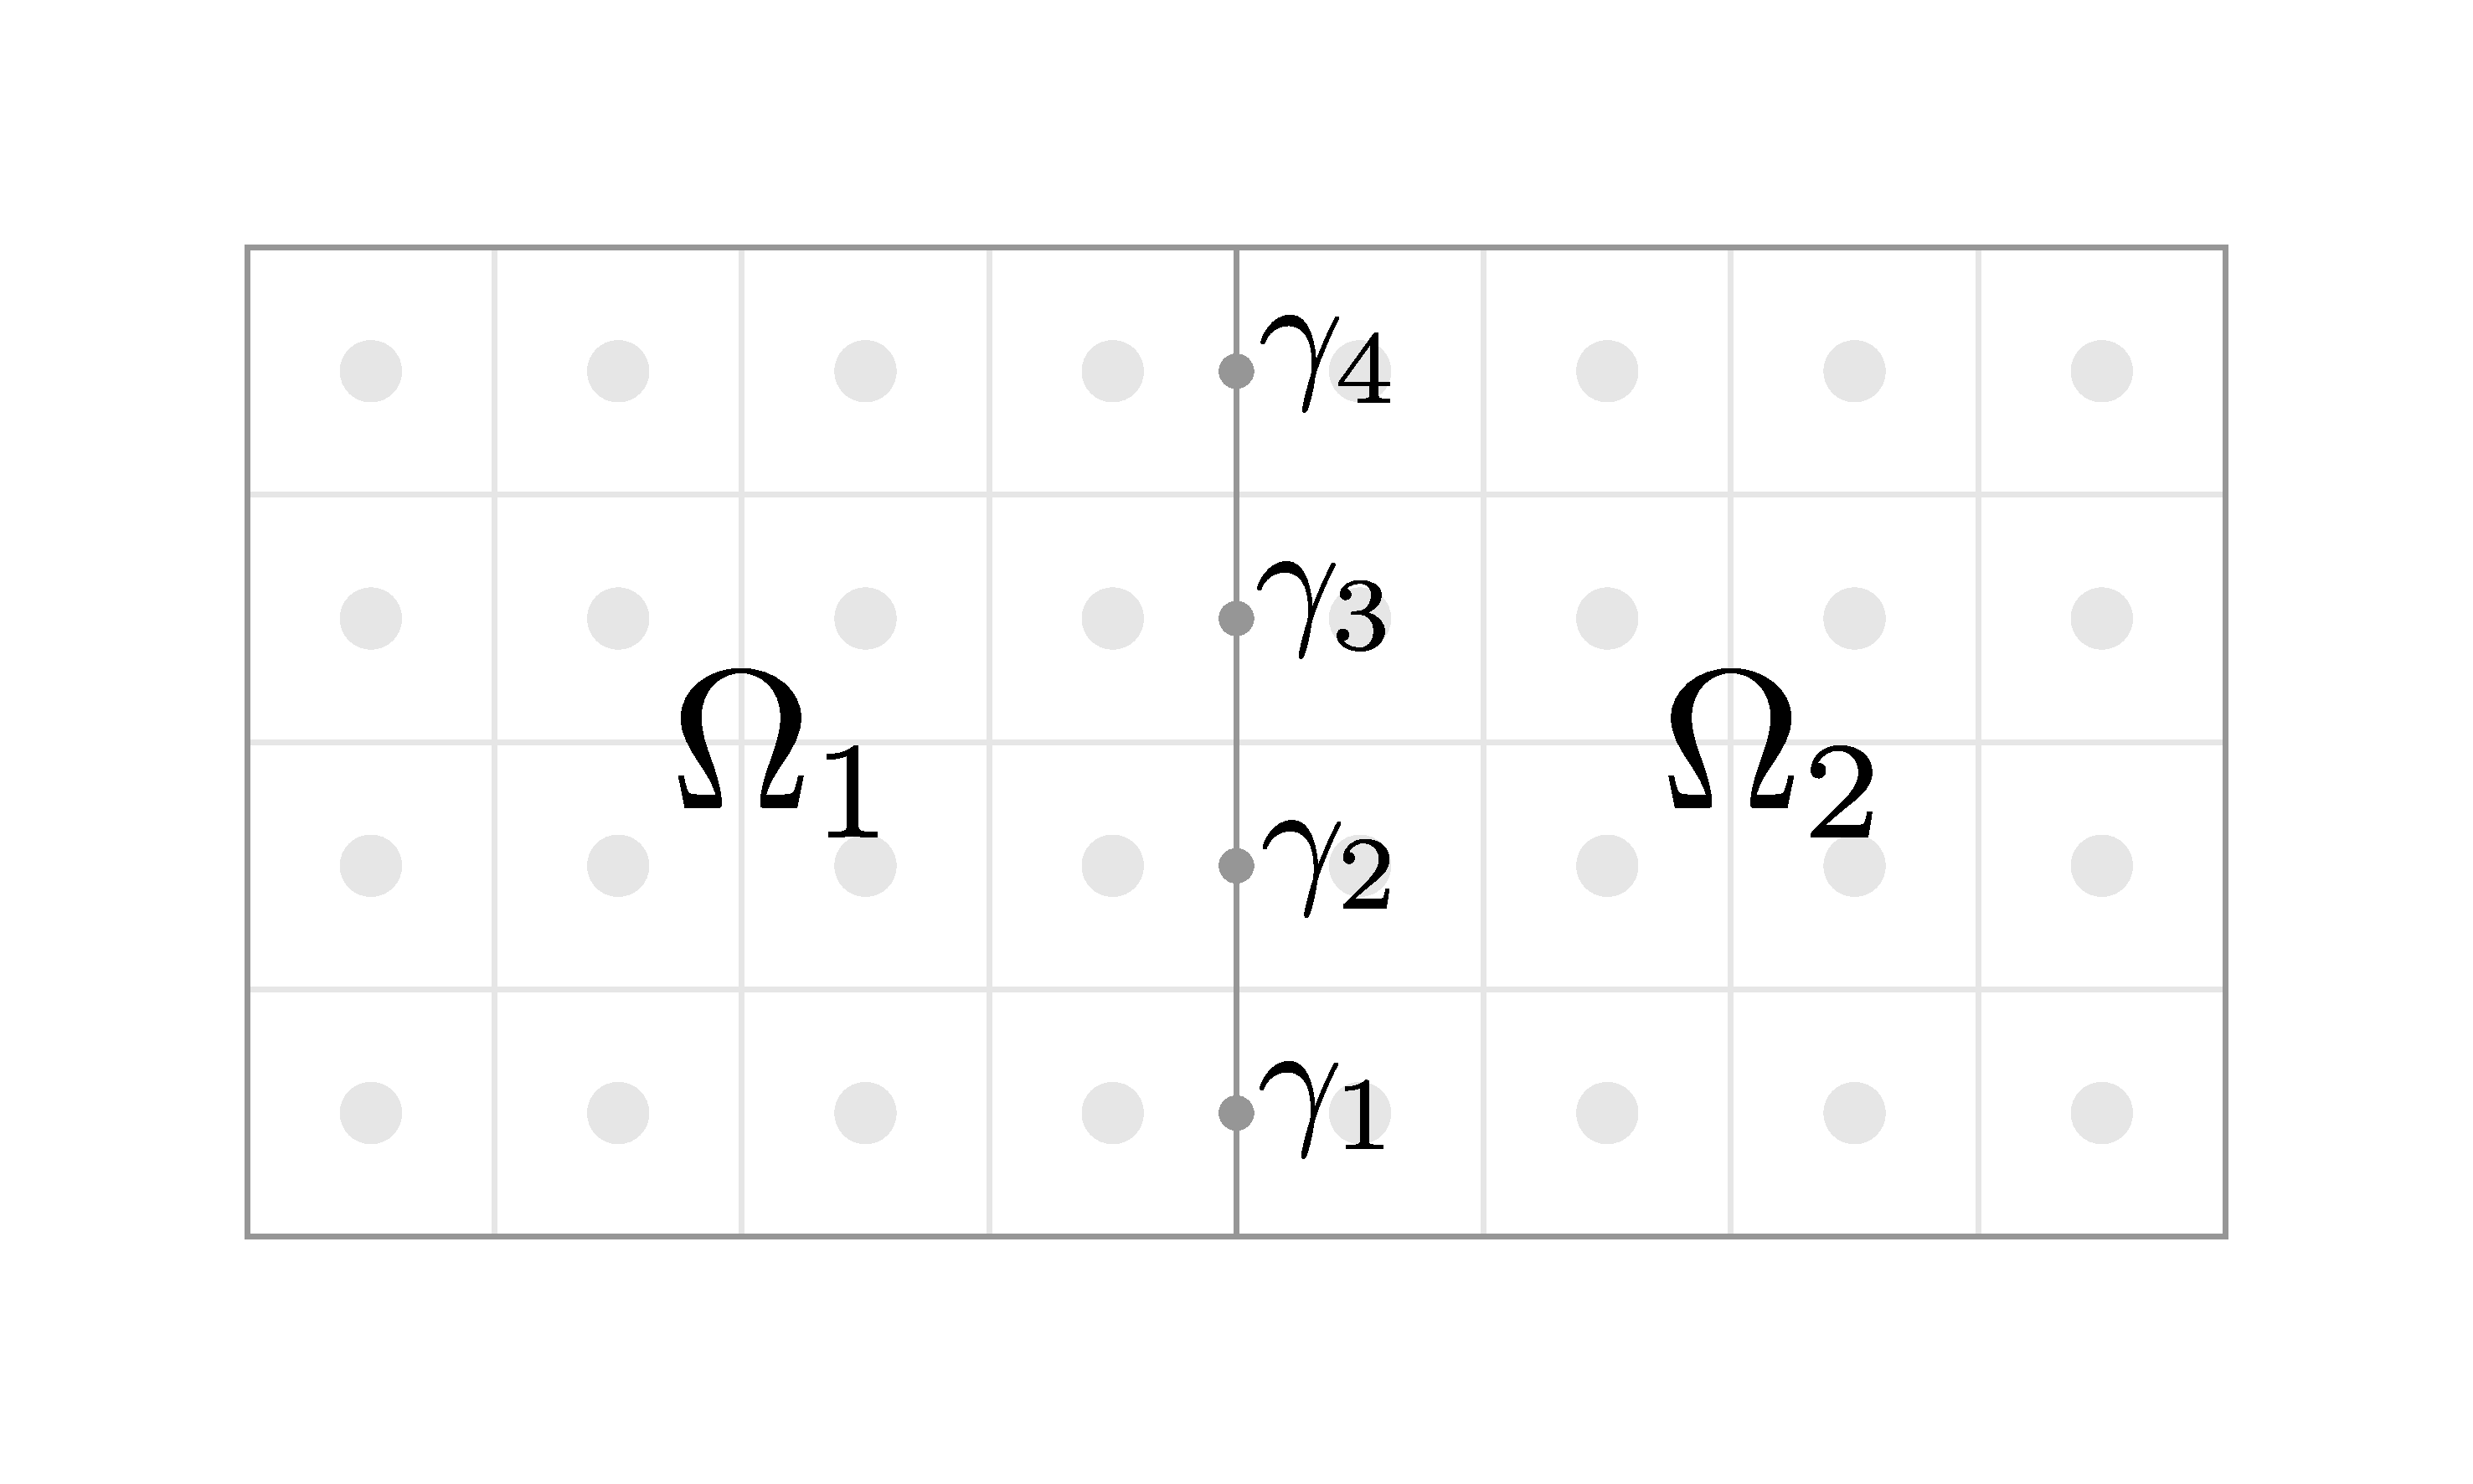
\includegraphics[width=4in]{images/abdomain.pdf}
    \caption{Two domain example}
\end{figure}
We want the gamma value to equal to the average of the solution on both sides:
\begin{equation}
    \gamma = \frac{East(\Omega_1)+West(\Omega_2)}{2}
\end{equation}
Where $East$ and $West$ are subroutines that return the solution values along the east side or west side
of a domain.
So now we have a function of $\gamma$
\begin{equation}
    F(\gamma)=2\gamma-(East(\Omega_1)+West(\Omega_2))
    \label{function}
\end{equation}
that we want to find the zero of. In subroutine form, this would look like:
\begin{algorithm}[H]
\caption{Two-Domain Function}
\begin{algorithmic}[1]
    \Procedure{F}{$\gamma$}
    \State $\Omega_1.solveWithInterface(\gamma)$
    \State $result \gets \gamma - \Omega_1.getSolutionEdge(East)$
    \State $\Omega_2.solveWithInterface(\gamma)$
    \State $result \gets result + \gamma - \Omega_2.getSolutionEdge(West)$
    \State \Return $result$
    \EndProcedure
\end{algorithmic}
\end{algorithm}

When there are multiple interface points, then we have a system of linear equations
\begin{equation}
F(\gamma)=A\gamma-b
\end{equation}
The $b$ vector is found by
\begin{equation}
b=-F(0)
    \label{bvec}
\end{equation}
and each column of the matrix is found by
\begin{equation}
A(:,i) = F(e_i)+b
    \label{matrixcol}
\end{equation}
we can then determine the  $\gamma$ vector by solving
\begin{equation}
A\gamma=b
\end{equation}
\subsection{Generalized Function}
Given some arbitrary mesh, we want to be able to index the interface values in the $\gamma$ vector.
One way that we can do this is have the interface values on each interface be consecutively indexed,
and also give a unique index to each of the interface. If our domains each have $n \times n$ values,
the interface with index $1$ will have the first $n$ values, a interface with index $2$ will have
the second $n$ values, and so on.

\paragraph{Indexing of Interfaces}
\begin{figure}
    \centering
    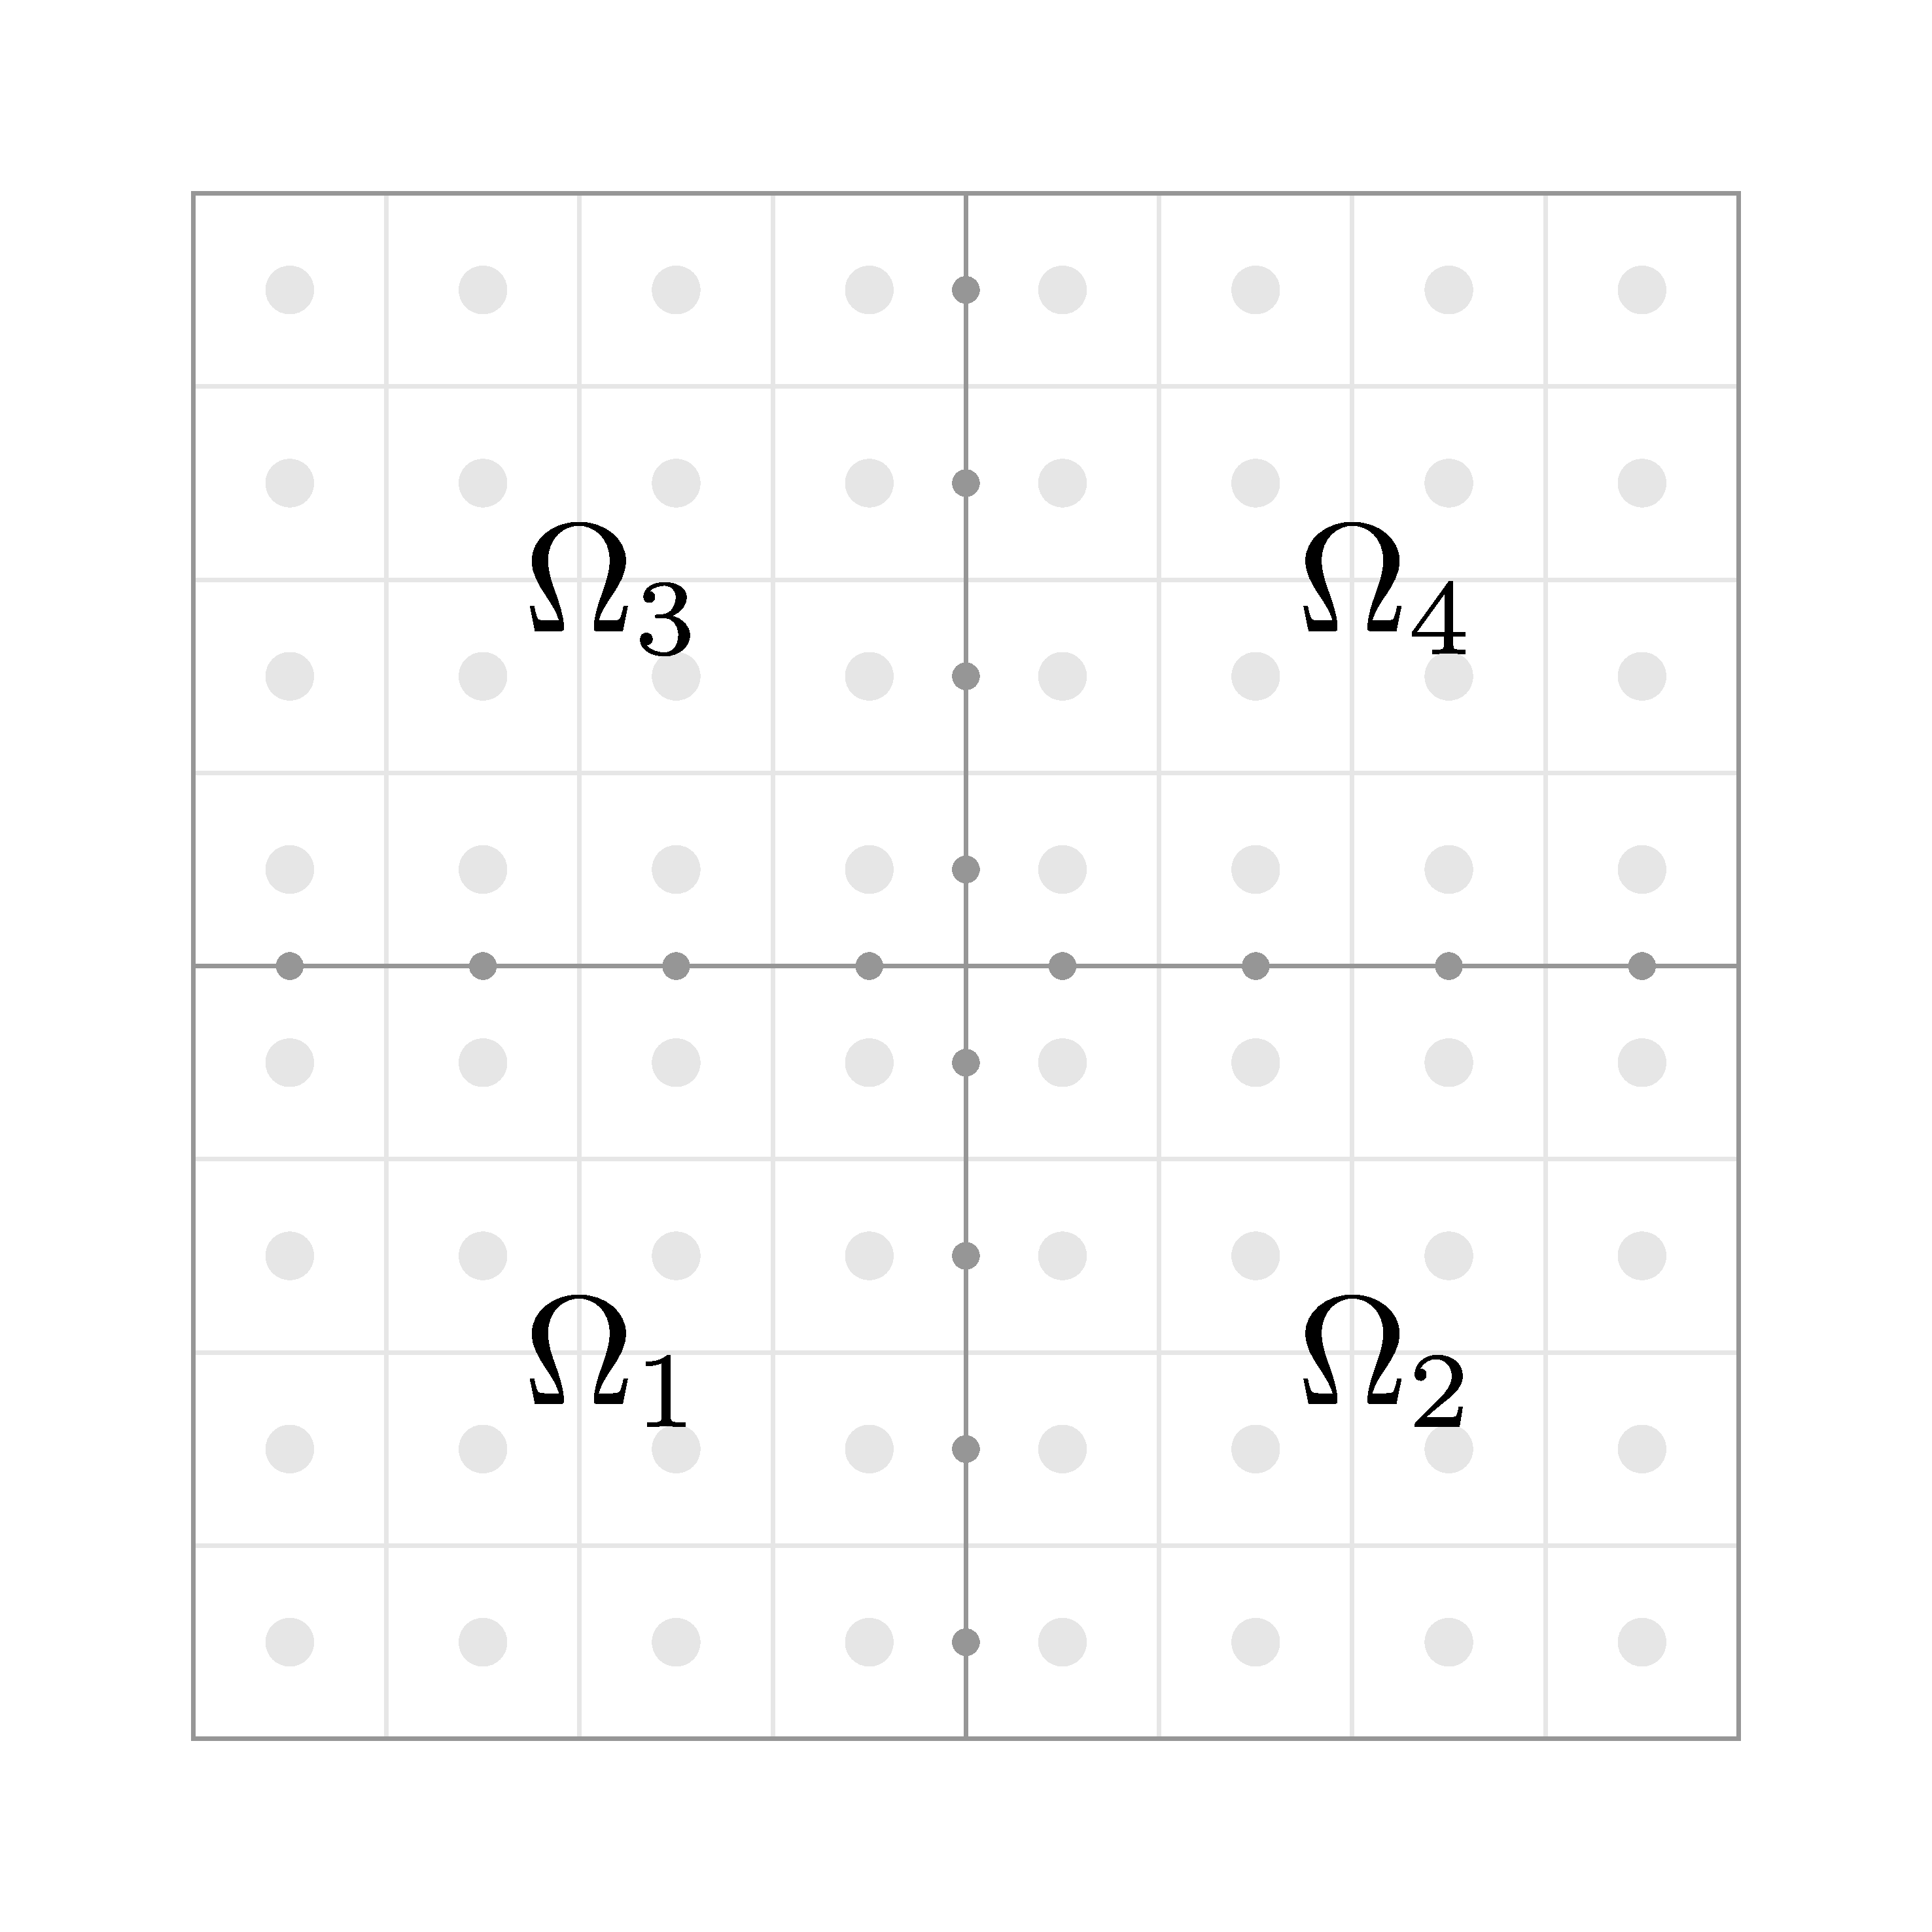
\includegraphics[width=3in]{images/4domain.pdf}
    \caption{Four domain mesh}
    \label{fourdomain}
\end{figure}
\begin{figure}
    \centering
    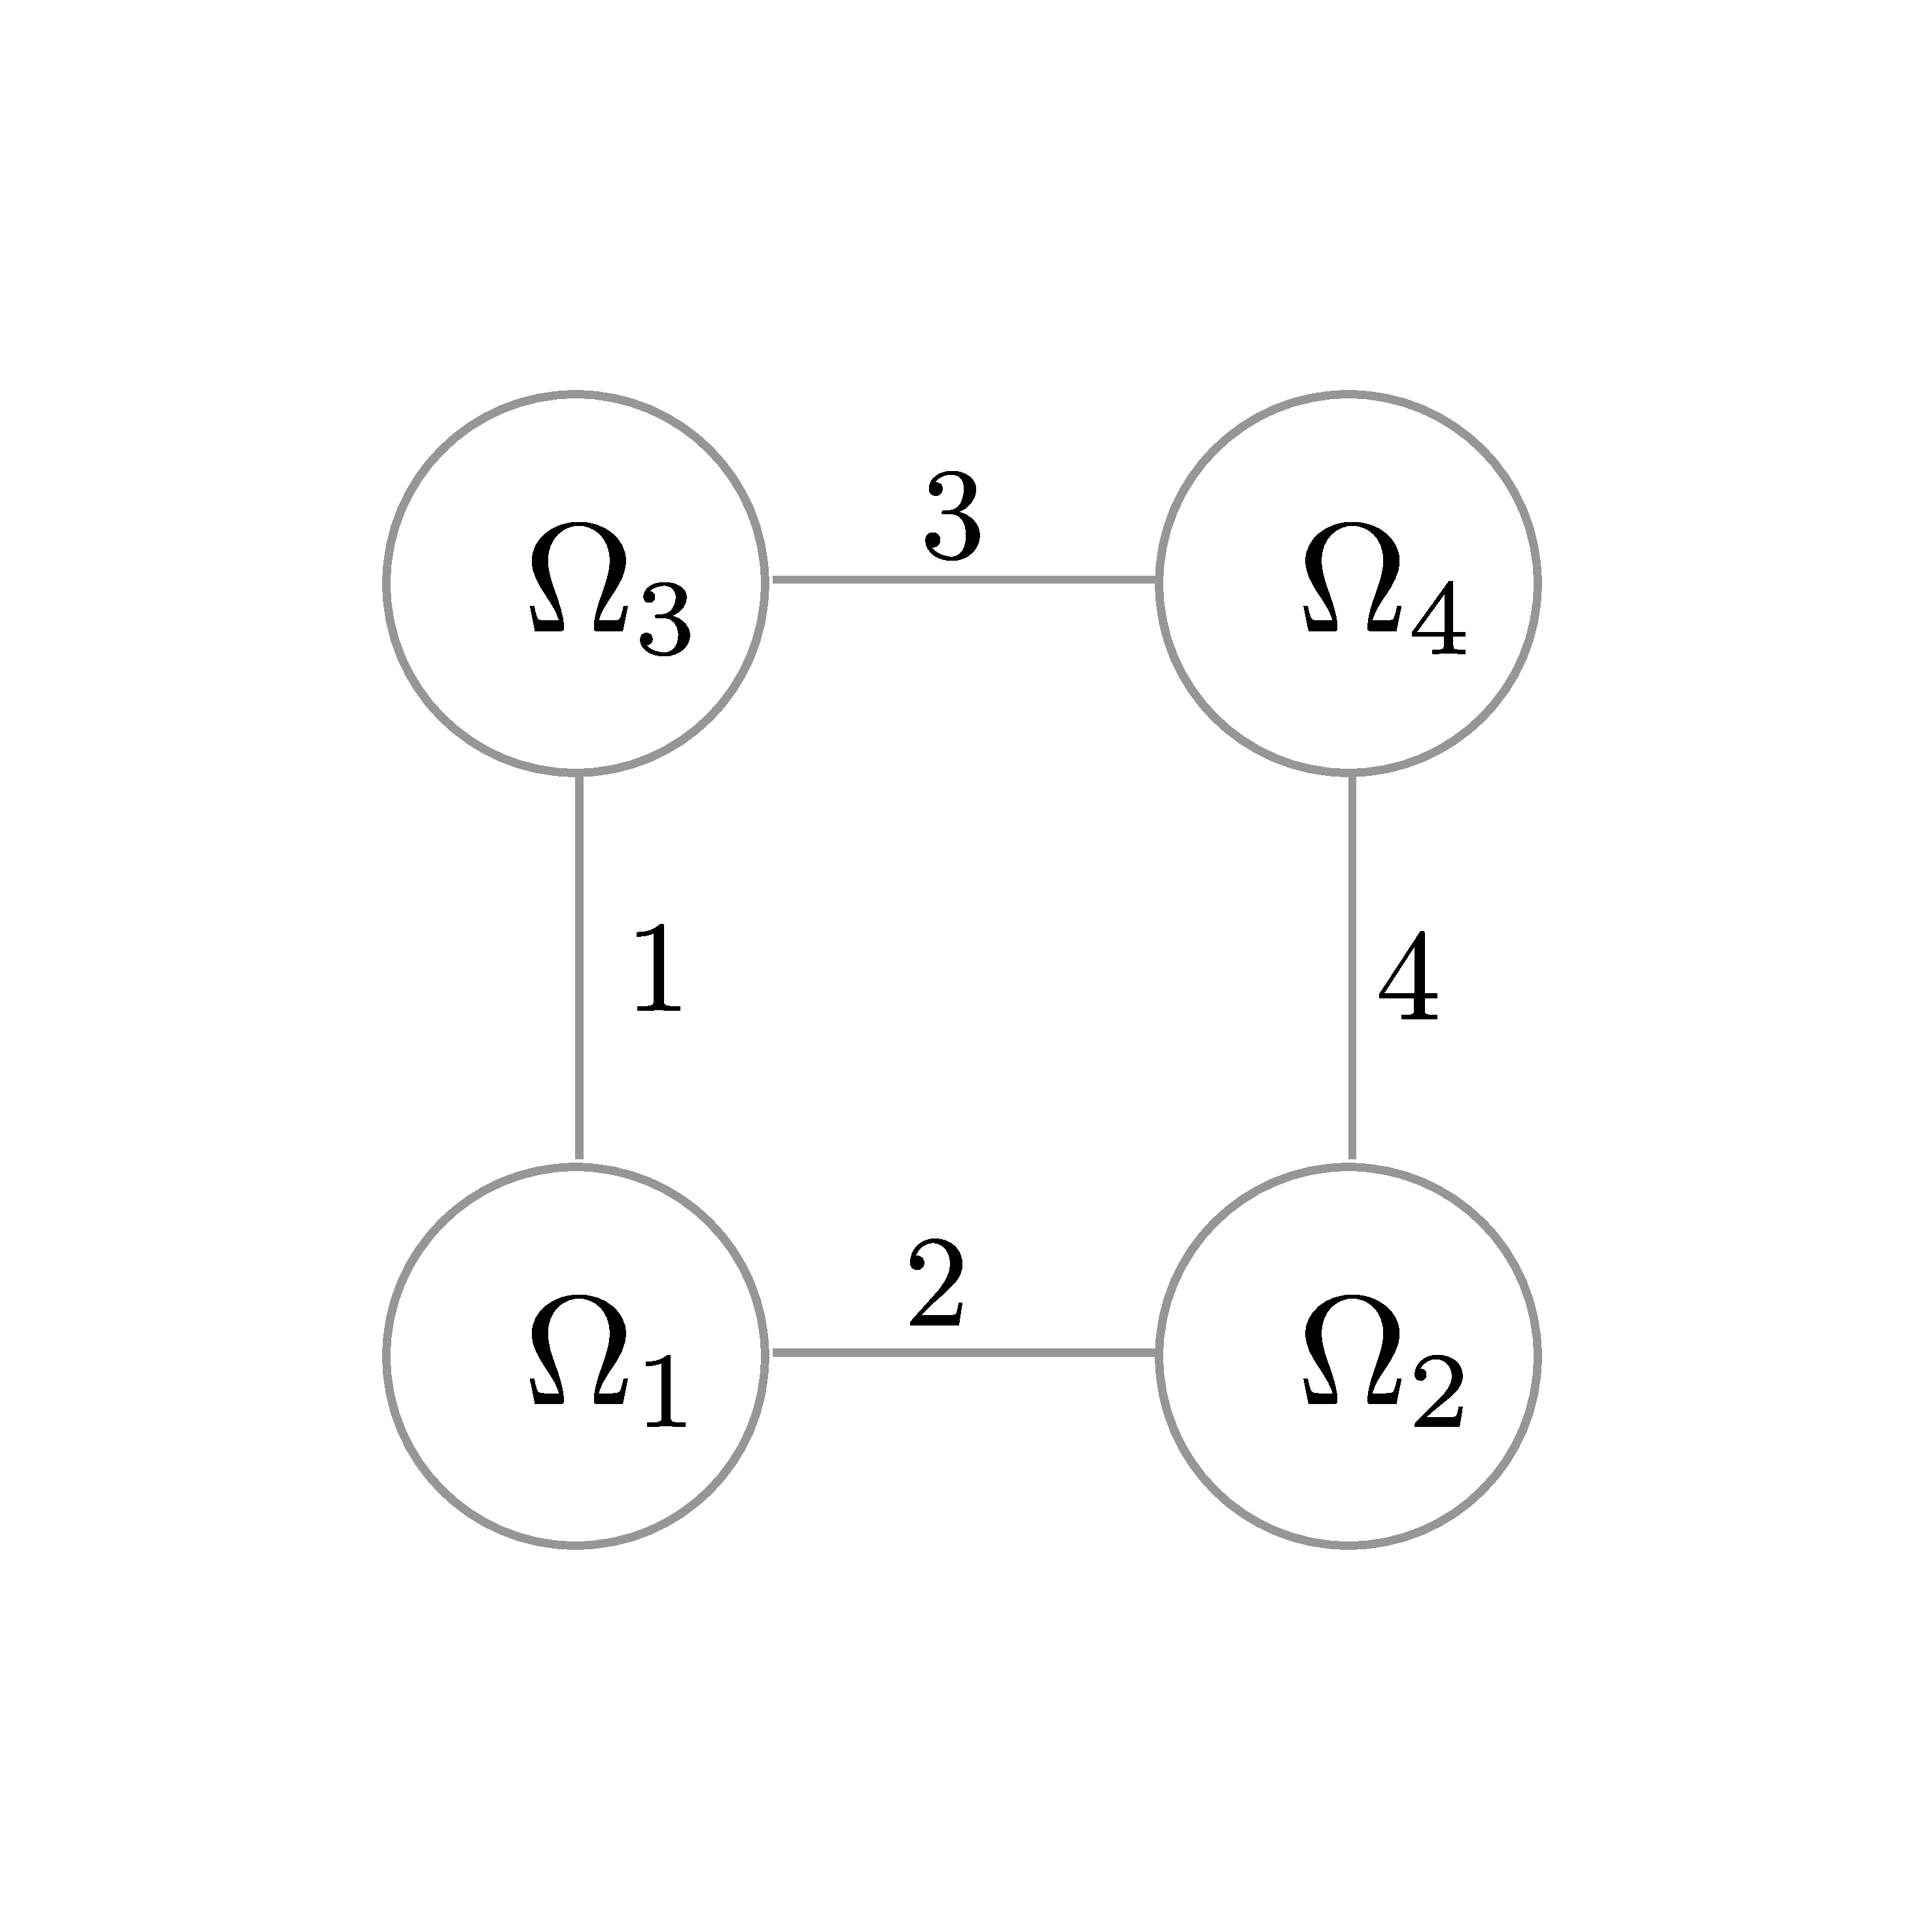
\includegraphics[width=3in]{images/4domaingraph.pdf}
    \caption{Indexing of interfaces}
    \label{fourgraph}
\end{figure}
Consider the mesh given in figure \ref{fourdomain}. In order to give a unique index to each
interface, we can think of the mesh as a graph. Where each domain is a vertex, and an edge 
represents
domains sharing an interface. We can then perform a breadth-first traversal of the graph and label
each edge with a unique index as is shown in figure \ref{fourgraph}. An algorithm for indexing the
interfaces is shown in algorithm \ref{indexbfs}. 

\begin{algorithm}[H]
\caption{Interface Indexing}
\begin{algorithmic}[1]
    \Procedure{IndexInterfacesBFS}{$\Omega_{start}$}
    \State $queue()$ \Comment{queue of domains to visit next}
    \State $queue.pushBack(\Omega_{start})$ \Comment{insert starting domain}
    \State $visited \gets \emptyset$ \Comment{set of visited domains}
    \State $i \gets 1$ 
    \While{$!queue.empty()$} \Comment{Breadth-First traversal of our mesh}
        \State $\Omega \gets queue.popFront()$
        \For{$side \in \{North,East,South,West\}$}
            \If{$\Omega.hasNeighbor(side)$ \textbf{and} $\Omega.getNeighbor(side) \notin visited$}
                \State $\Omega_{nbr} \gets \Omega.getNeighbor(side)$
                \If{$\Omega_{nbr}\notin queue$}
                    \State $queue.pushBack(\Omega_{nbr})$
                \EndIf
                \State $\Omega.ifaceIndex(side)\gets i$ \Comment{Set index for interface}
                \State $\Omega_{nbr}.ifaceIndex(Opposite(side))\gets i$ \Comment{Also set index for
                neighbor}
                \State $i \gets i+1$
            \EndIf
        \EndFor
        \State $visited.insert(\Omega)$
    \EndWhile
    \EndProcedure
\end{algorithmic}
\label{indexbfs}
\end{algorithm}

\paragraph{Consecutive Indexing of $\gamma$ Values} 
We can index the values on each interface in the following way:
\begin{itemize}
    \item If the interface is on the east or west side of the patch, the $\gamma$ values will be indexed consecutively from the bottom up.
    \item If the interface is on the north or south side of the patch, the $\gamma$ values will be indexed consecutively from left to right.
\end{itemize}
\begin{figure}
    \label{indexing}
    \centering
    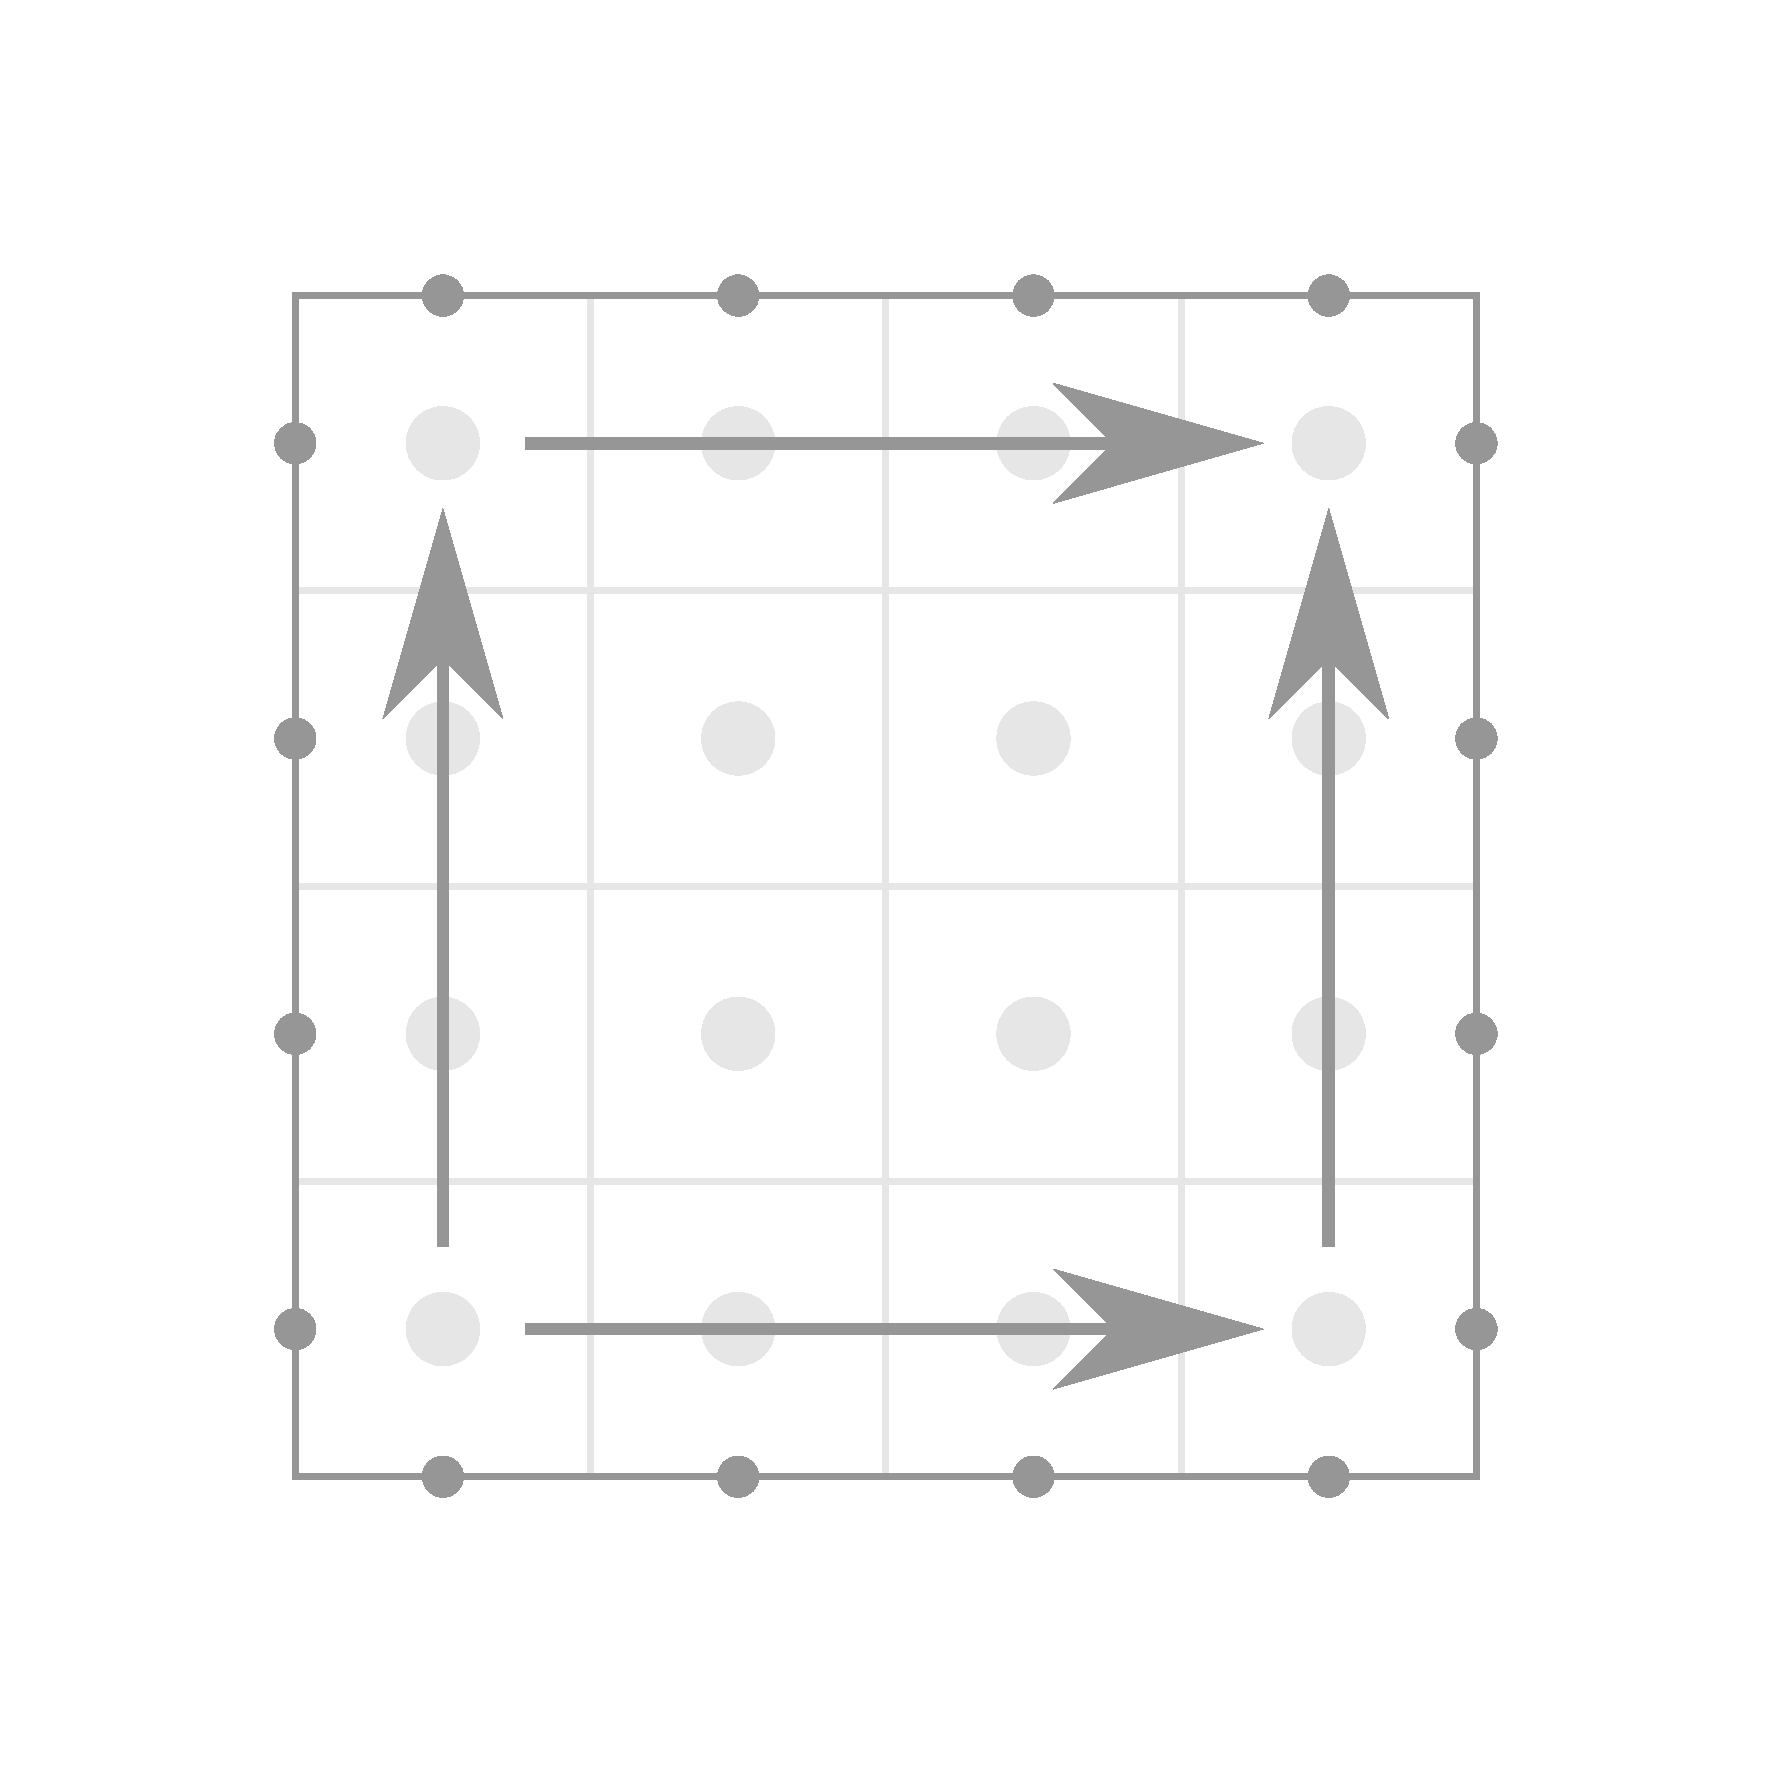
\includegraphics[width=3in]{images/indexing.pdf}
    \caption{Graph of four domain mesh}
\end{figure}
Since the $\gamma$ values on each interface indexed consecutively, the Schur complement matrix takes
on a block structure, where each block is $n\times n$.

\paragraph{Generalized Function} 
Once each interface vlaue has an index, we can use algorithm \ref{genfunc} for the function that we
want to find the zero of.
\begin{algorithm}[H]
\caption{Generalized Function}
\begin{algorithmic}[1]
    \Procedure{F}{$\gamma, Domains$}
    \State $result(\gamma.size())$ \Comment{Allocate new vector}
    \For{$\Omega \in Domains$}
        \State $\Omega.solveWithInterface(\gamma)$
        \For{$side \in \{North,East,South,West\}$}
            \If{$\Omega.hasNeighbor(side)$}
                \State $i \gets \Omega.ifaceIndex(side)$
                \State $start \gets i*(n-1)+1$
                \State $stop \gets i*n$
                \State $result(start:stop) \gets \gamma(start:stop) - \Omega.getSolutionEdge(side)$
            \EndIf
        \EndFor
    \EndFor
    \State \Return $result$
    \EndProcedure
\end{algorithmic}
\label{genfunc}
\end{algorithm}

\section{Quick Formulation of the Schur Complement Matrix}
In this section, we can use the process described in equation \eqref{matrixcol} to derive an algorithm
that allow us to quickly form the Schur compliment matrix.
\paragraph{The matrix does not depent on the RHS on the domains}
First, let's reconsider equations  \eqref{bvec} and \eqref{matrixcol}. If we are solving on a system
where the solution zero, the $b$ vector for the Schur complement matrix will
be $0$, since $0$ is the correct solution for the interfaces. So equation \eqref{matrixcol} turns into
\begin{equation}
    A(:,i) = F_{zero}(e_i)
\end{equation}
where $F_{zero}$ is the same as equation \ref{function}, but instead we are solving a system where
the solution is zero.
So now we use can use this to reduce the amount of work needed to form the Schur complement matrix.
\\
\\
Let's consider what happens when we solve for $F_{zero}(e_i)$. If a single interface value is set
to $1$, only the two adjacent domains will have non-zero dirichlet boundary conditions, meaning that
only the two adjacent domains will have non-zero solutions. This means that when we are solving for 
$F_{zero}(e_i)$, we can  assume that solution on any domain that is not adjacent to the interface
with the $1$ is zero. In other words, we only have to do a solve on the two adjacent domains, rather
than solving for all the domains.

\paragraph{Sparsity}

Consider the example grid given in Figure \ref{2domain}.
When a single $1$ is set on the interface $i_{\textnormal{main}}$, only 7 interfaces will end up
having non-zero values: the main interface, $i_{\textnormal{main}}$, and the 6 auxiliary
interfaces, 
$i_{\textnormal{left north}}$, $i_{\textnormal{left south}}$, $i_{\textnormal{left west}}$,
$i_{\textnormal{right north}}$, $i_{\textnormal{right east}}$, and $i_{\textnormal{right south}}$.

For each 1 that is set along the main interface, the same 7 interface will return non-zero values.
This means that for each interface, there will be maximum of 7 blocks of size $n \times n$.
$$
A(:,j)=
\begin{bmatrix}
    \vdots \\
    \bullet\\
    \bullet\\
    \bullet\\
    \bullet\\
    \vdots \\
    \bullet\\
    \bullet\\
    \bullet\\
    \bullet\\
    \vdots \\
    \bullet\\
    \bullet\\
    \bullet\\
    \bullet\\
    \vdots \\
    \bullet\\
    \bullet\\
    \bullet\\
    \bullet\\
    \vdots \\
    \bullet\\
    \bullet\\
    \bullet\\
    \bullet\\
    \vdots \\
    \bullet\\
    \bullet\\
    \bullet\\
    \bullet\\
    \vdots \\
    \bullet\\
    \bullet\\
    \bullet\\
    \bullet\\
    \vdots \\
\end{bmatrix}
\qquad
A(:,j:(j+n))=
\begin{bmatrix}
    \vdots  & \vdots  & \vdots  & \vdots \\
    \bullet & \bullet & \bullet & \bullet \\
    \bullet & \bullet & \bullet & \bullet \\
    \bullet & \bullet & \bullet & \bullet \\
    \bullet & \bullet & \bullet & \bullet \\
    \vdots  & \vdots  & \vdots  & \vdots \\
    \bullet & \bullet & \bullet & \bullet \\
    \bullet & \bullet & \bullet & \bullet \\
    \bullet & \bullet & \bullet & \bullet \\
    \bullet & \bullet & \bullet & \bullet \\
    \vdots  & \vdots  & \vdots  & \vdots \\
    \bullet & \bullet & \bullet & \bullet \\
    \bullet & \bullet & \bullet & \bullet \\
    \bullet & \bullet & \bullet & \bullet \\
    \bullet & \bullet & \bullet & \bullet \\
    \vdots  & \vdots  & \vdots  & \vdots \\
    \bullet & \bullet & \bullet & \bullet \\
    \bullet & \bullet & \bullet & \bullet \\
    \bullet & \bullet & \bullet & \bullet \\
    \bullet & \bullet & \bullet & \bullet \\
    \vdots  & \vdots  & \vdots  & \vdots \\
    \bullet & \bullet & \bullet & \bullet \\
    \bullet & \bullet & \bullet & \bullet \\
    \bullet & \bullet & \bullet & \bullet \\
    \bullet & \bullet & \bullet & \bullet \\
    \vdots  & \vdots  & \vdots  & \vdots \\
    \bullet & \bullet & \bullet & \bullet \\
    \bullet & \bullet & \bullet & \bullet \\
    \bullet & \bullet & \bullet & \bullet \\
    \bullet & \bullet & \bullet & \bullet \\
    \vdots  & \vdots  & \vdots  & \vdots \\
    \bullet & \bullet & \bullet & \bullet \\
    \bullet & \bullet & \bullet & \bullet \\
    \bullet & \bullet & \bullet & \bullet \\
    \bullet & \bullet & \bullet & \bullet \\
    \vdots  & \vdots  & \vdots  & \vdots \\
\end{bmatrix}
$$
\begin{figure}[H]
    \centering
    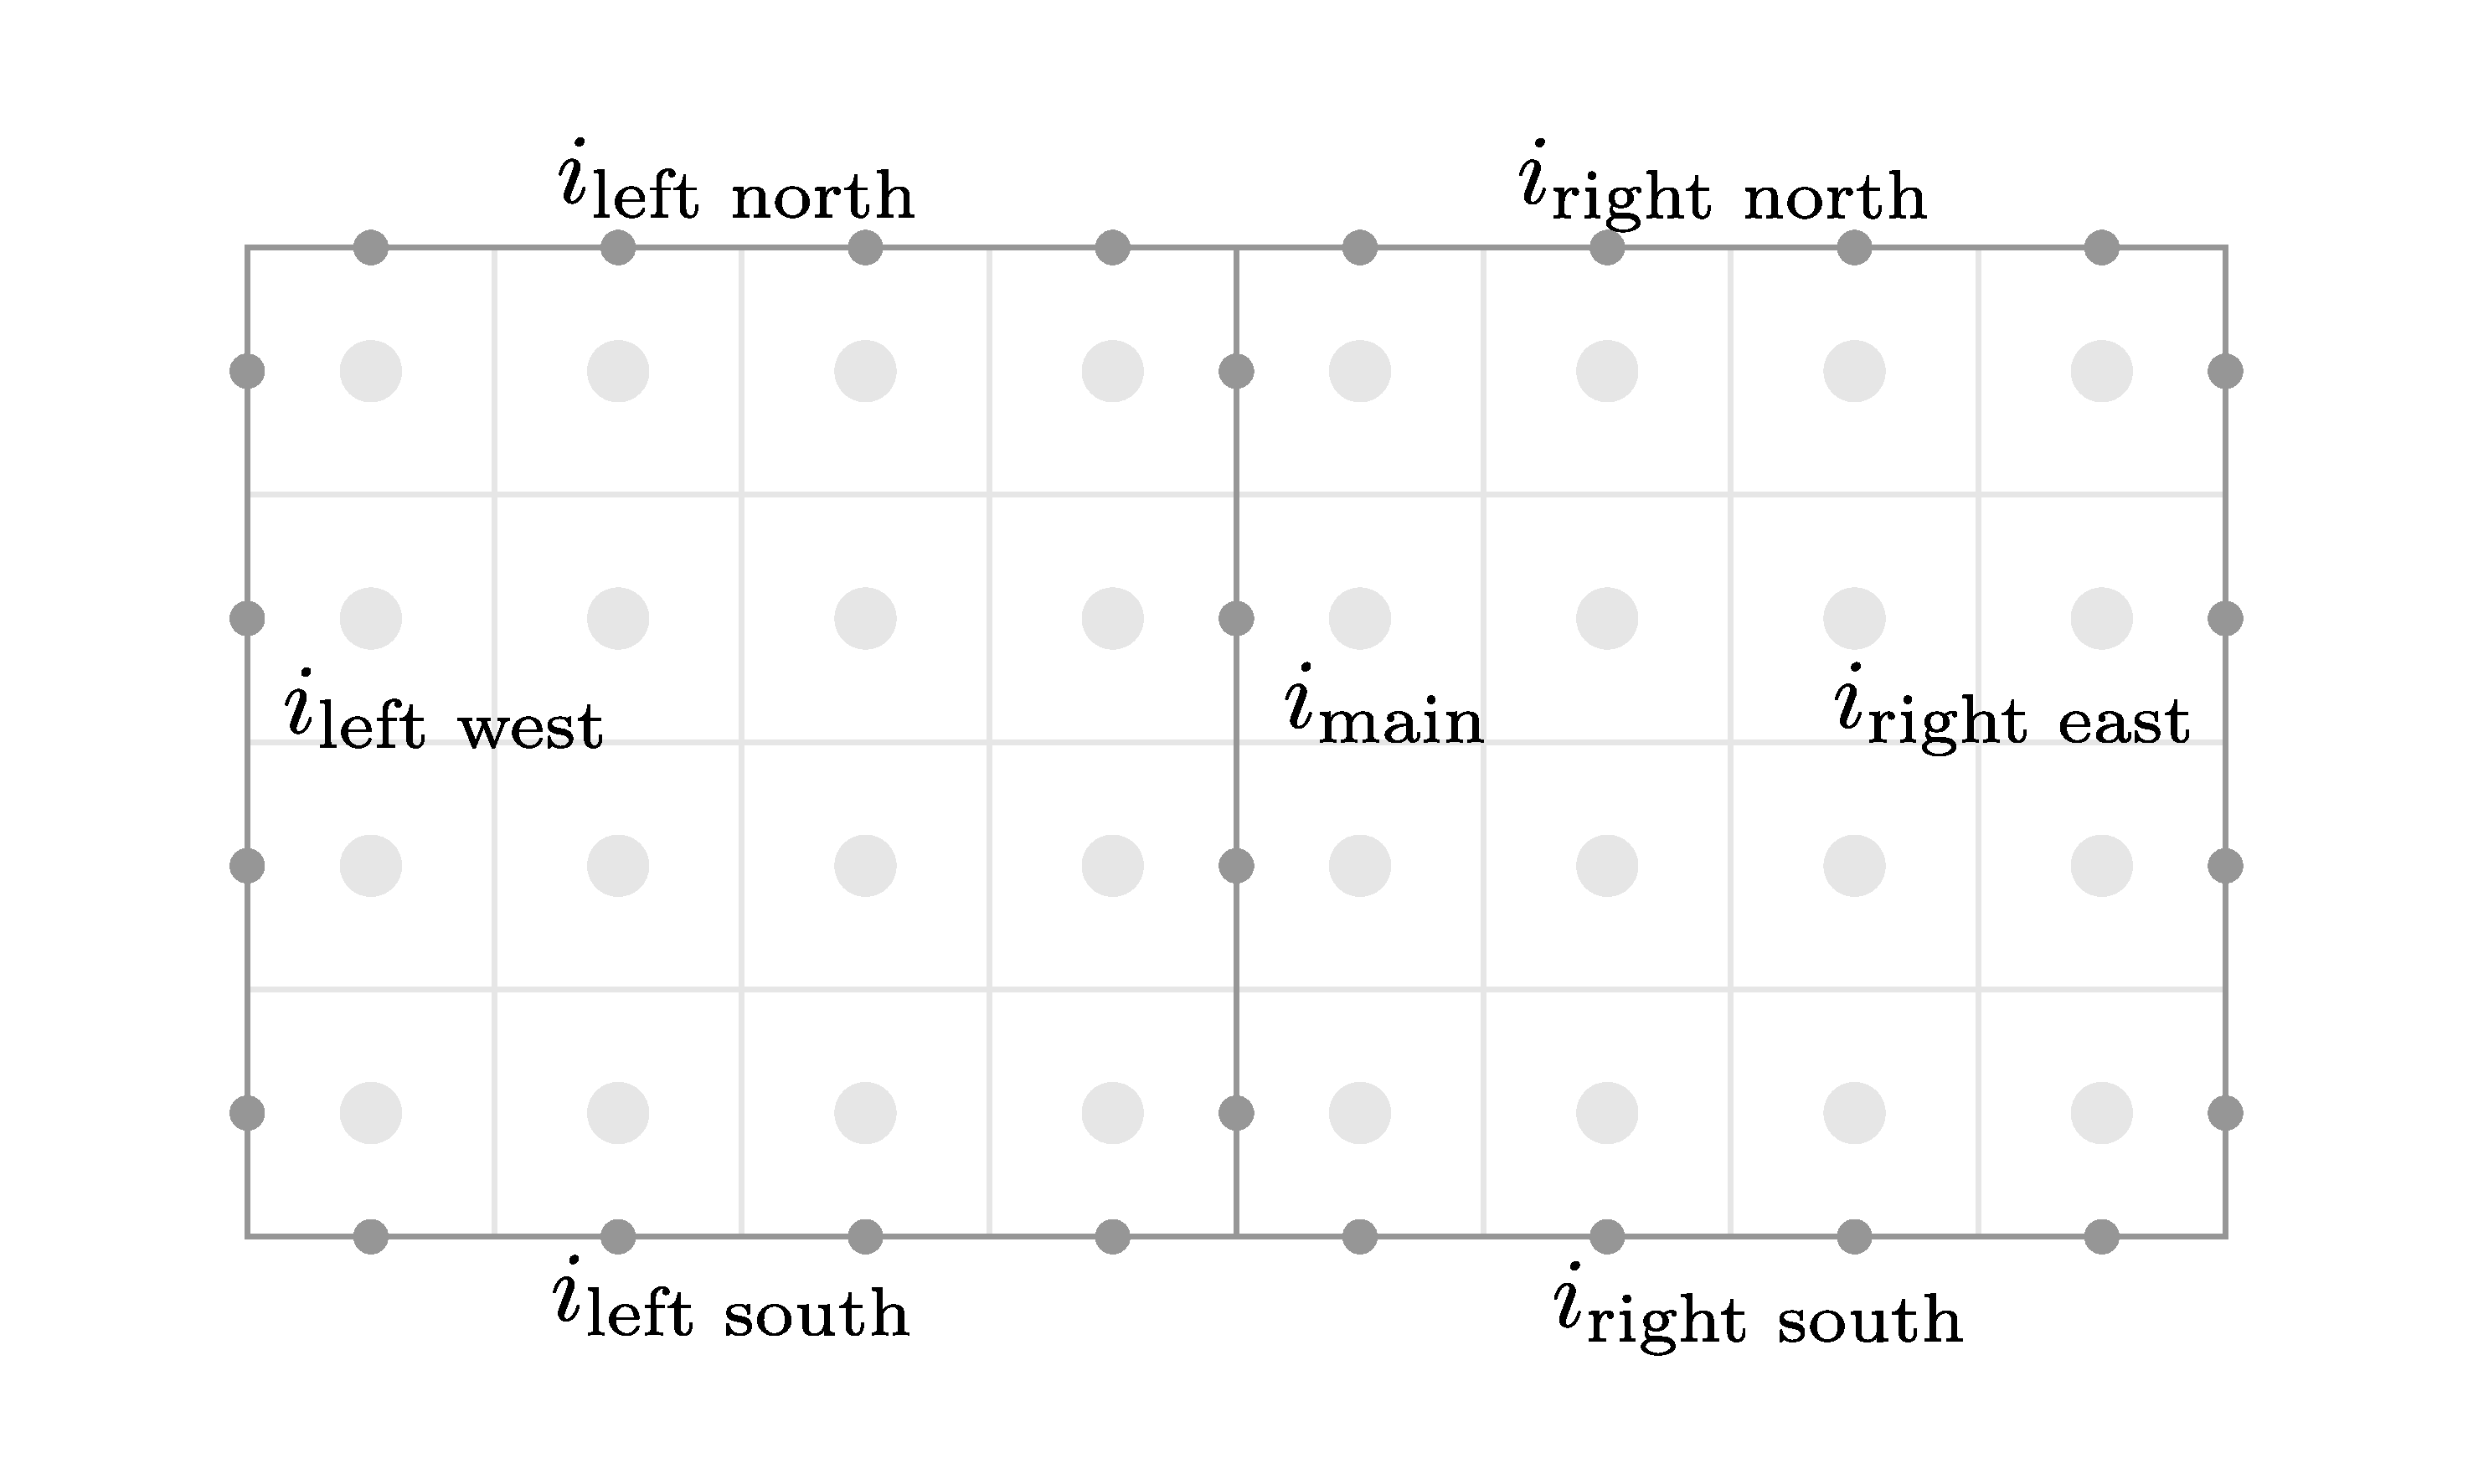
\includegraphics[width=6in]{images/2domain.pdf}
    \caption{Two domain example}
    \label{2domain}
\end{figure}

%\paragraph{Splitting up the work}
%
%If we look at equation \ref{function}, we can split up the work and process the two domains at
%different times.
%\begin{align}
%    F_{left}(\gamma)&=\gamma-L(\gamma) \label{function_left}\\
%    F_{right}(\gamma)&=\gamma-R(\gamma) \label{function_right}
%\end{align}
%
%So, when we process the left and right domains, we use equations \eqref{function_left} and 
%\eqref{function_right}, respectively, for the diagonal blocks ($i_{\textnormal{main}}$).
%When we are forming the matrix, we will insert the diagonal
%block twice, summing the coefficients of one block into the other.

\paragraph{Rotation}
\begin{figure}
    \centering
    \begin{subfigure}[b]{0.30\textwidth}
        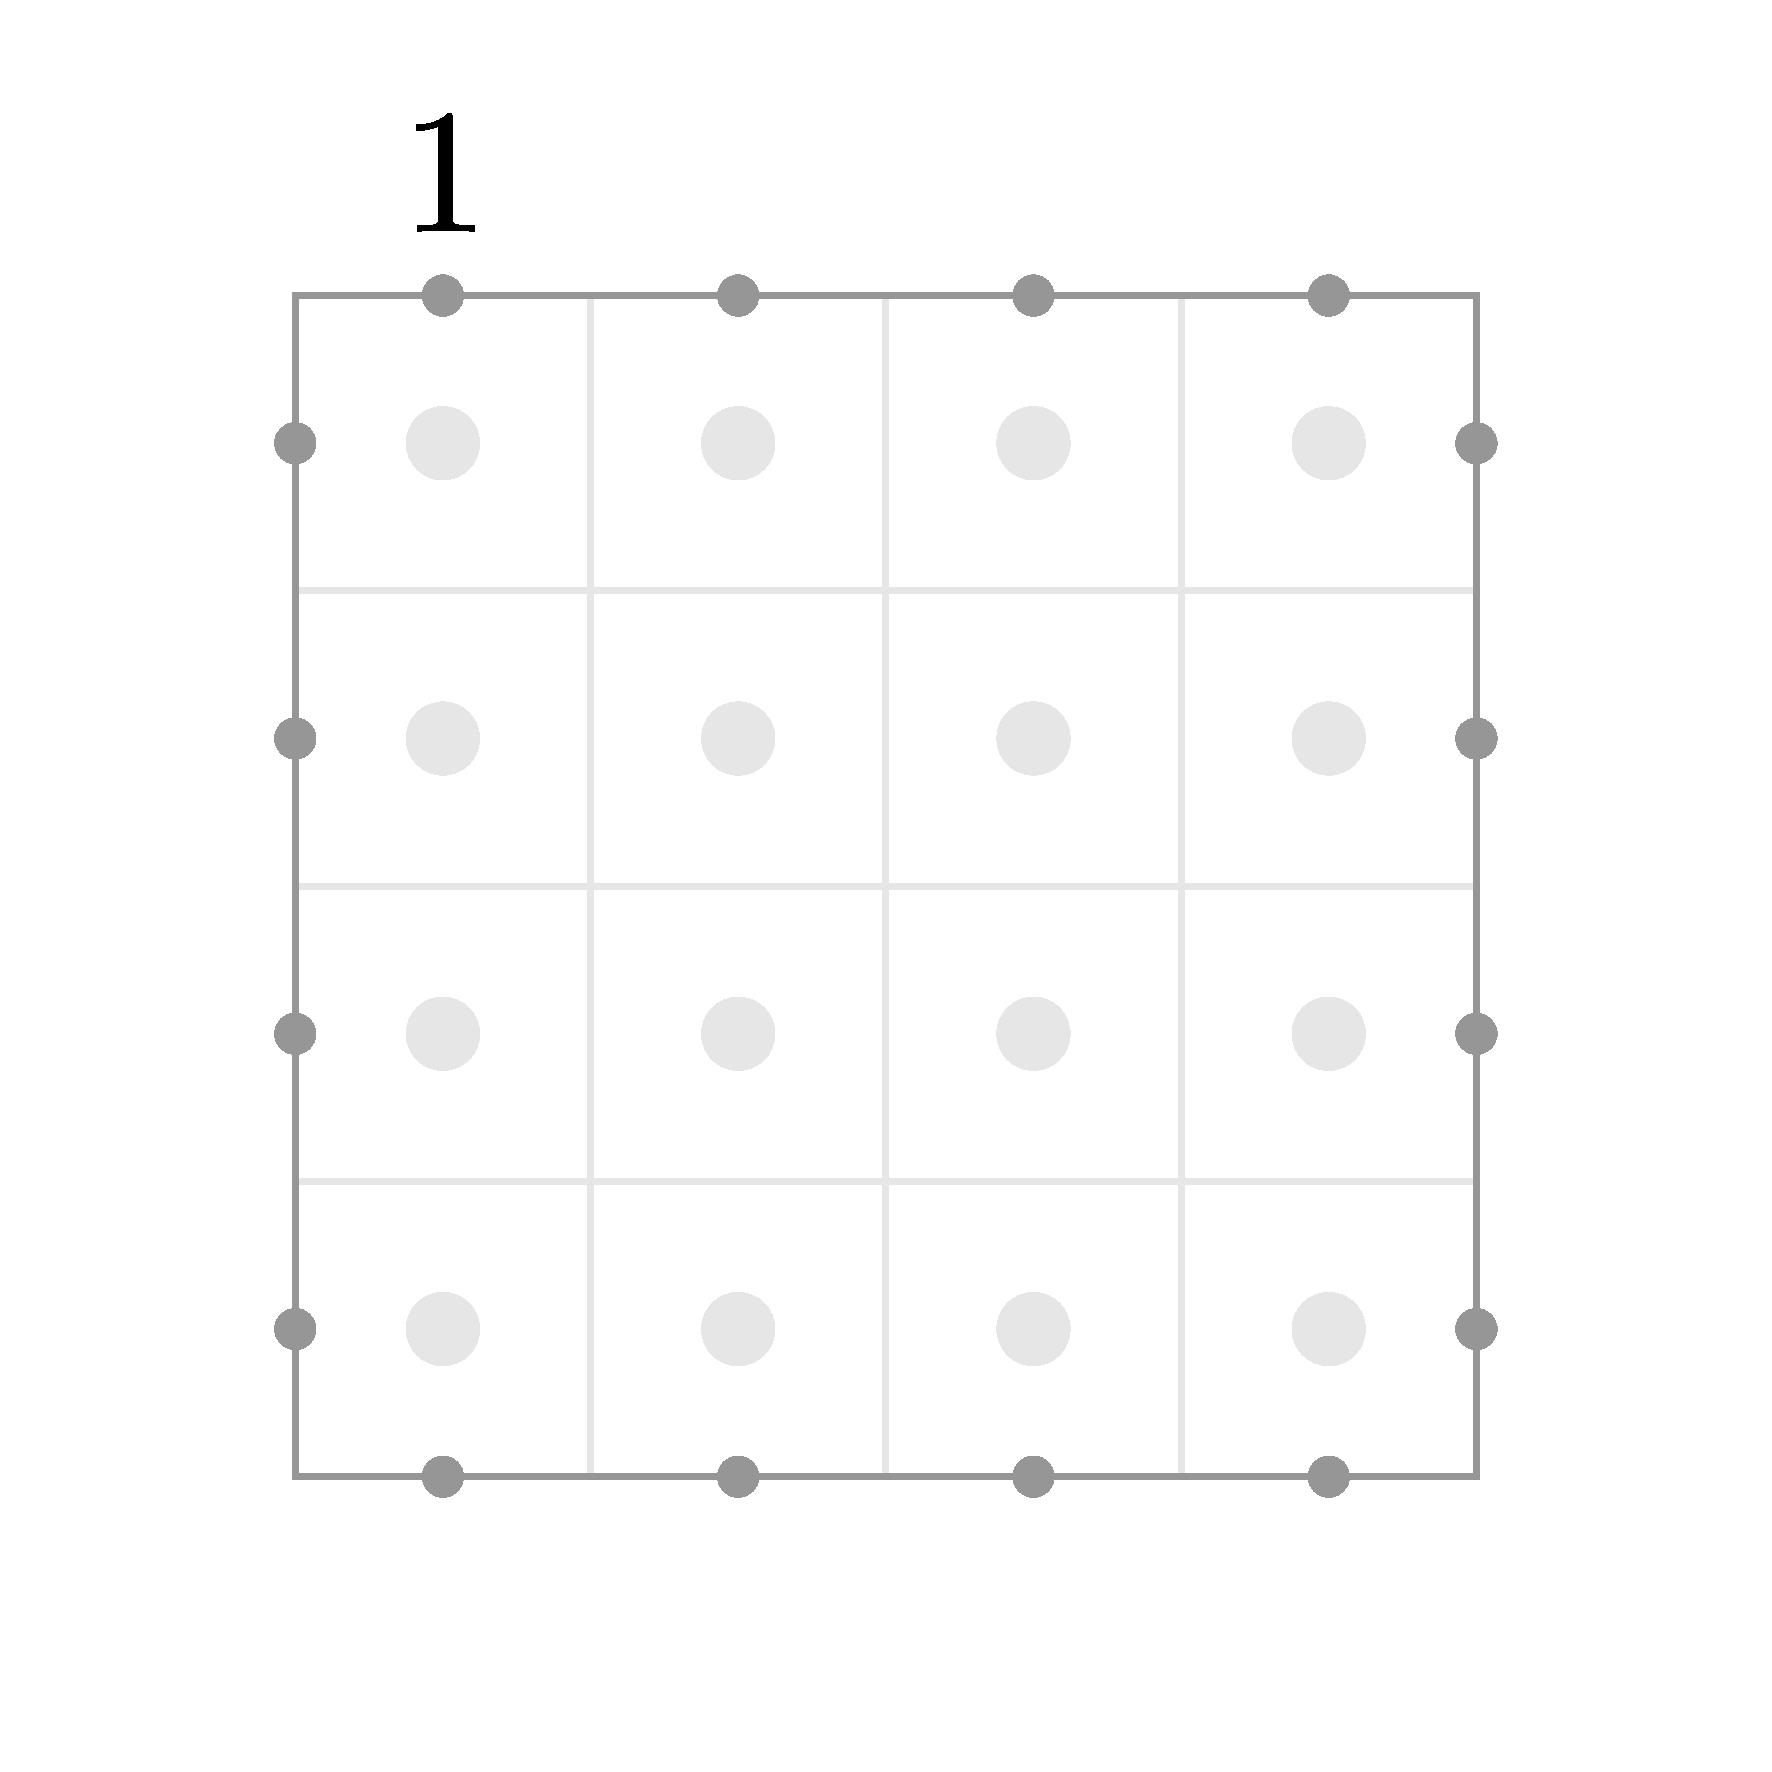
\includegraphics[width=\textwidth]{images/north1.pdf}
        \caption{North}
    \end{subfigure}
    \begin{subfigure}[b]{0.30\textwidth}
        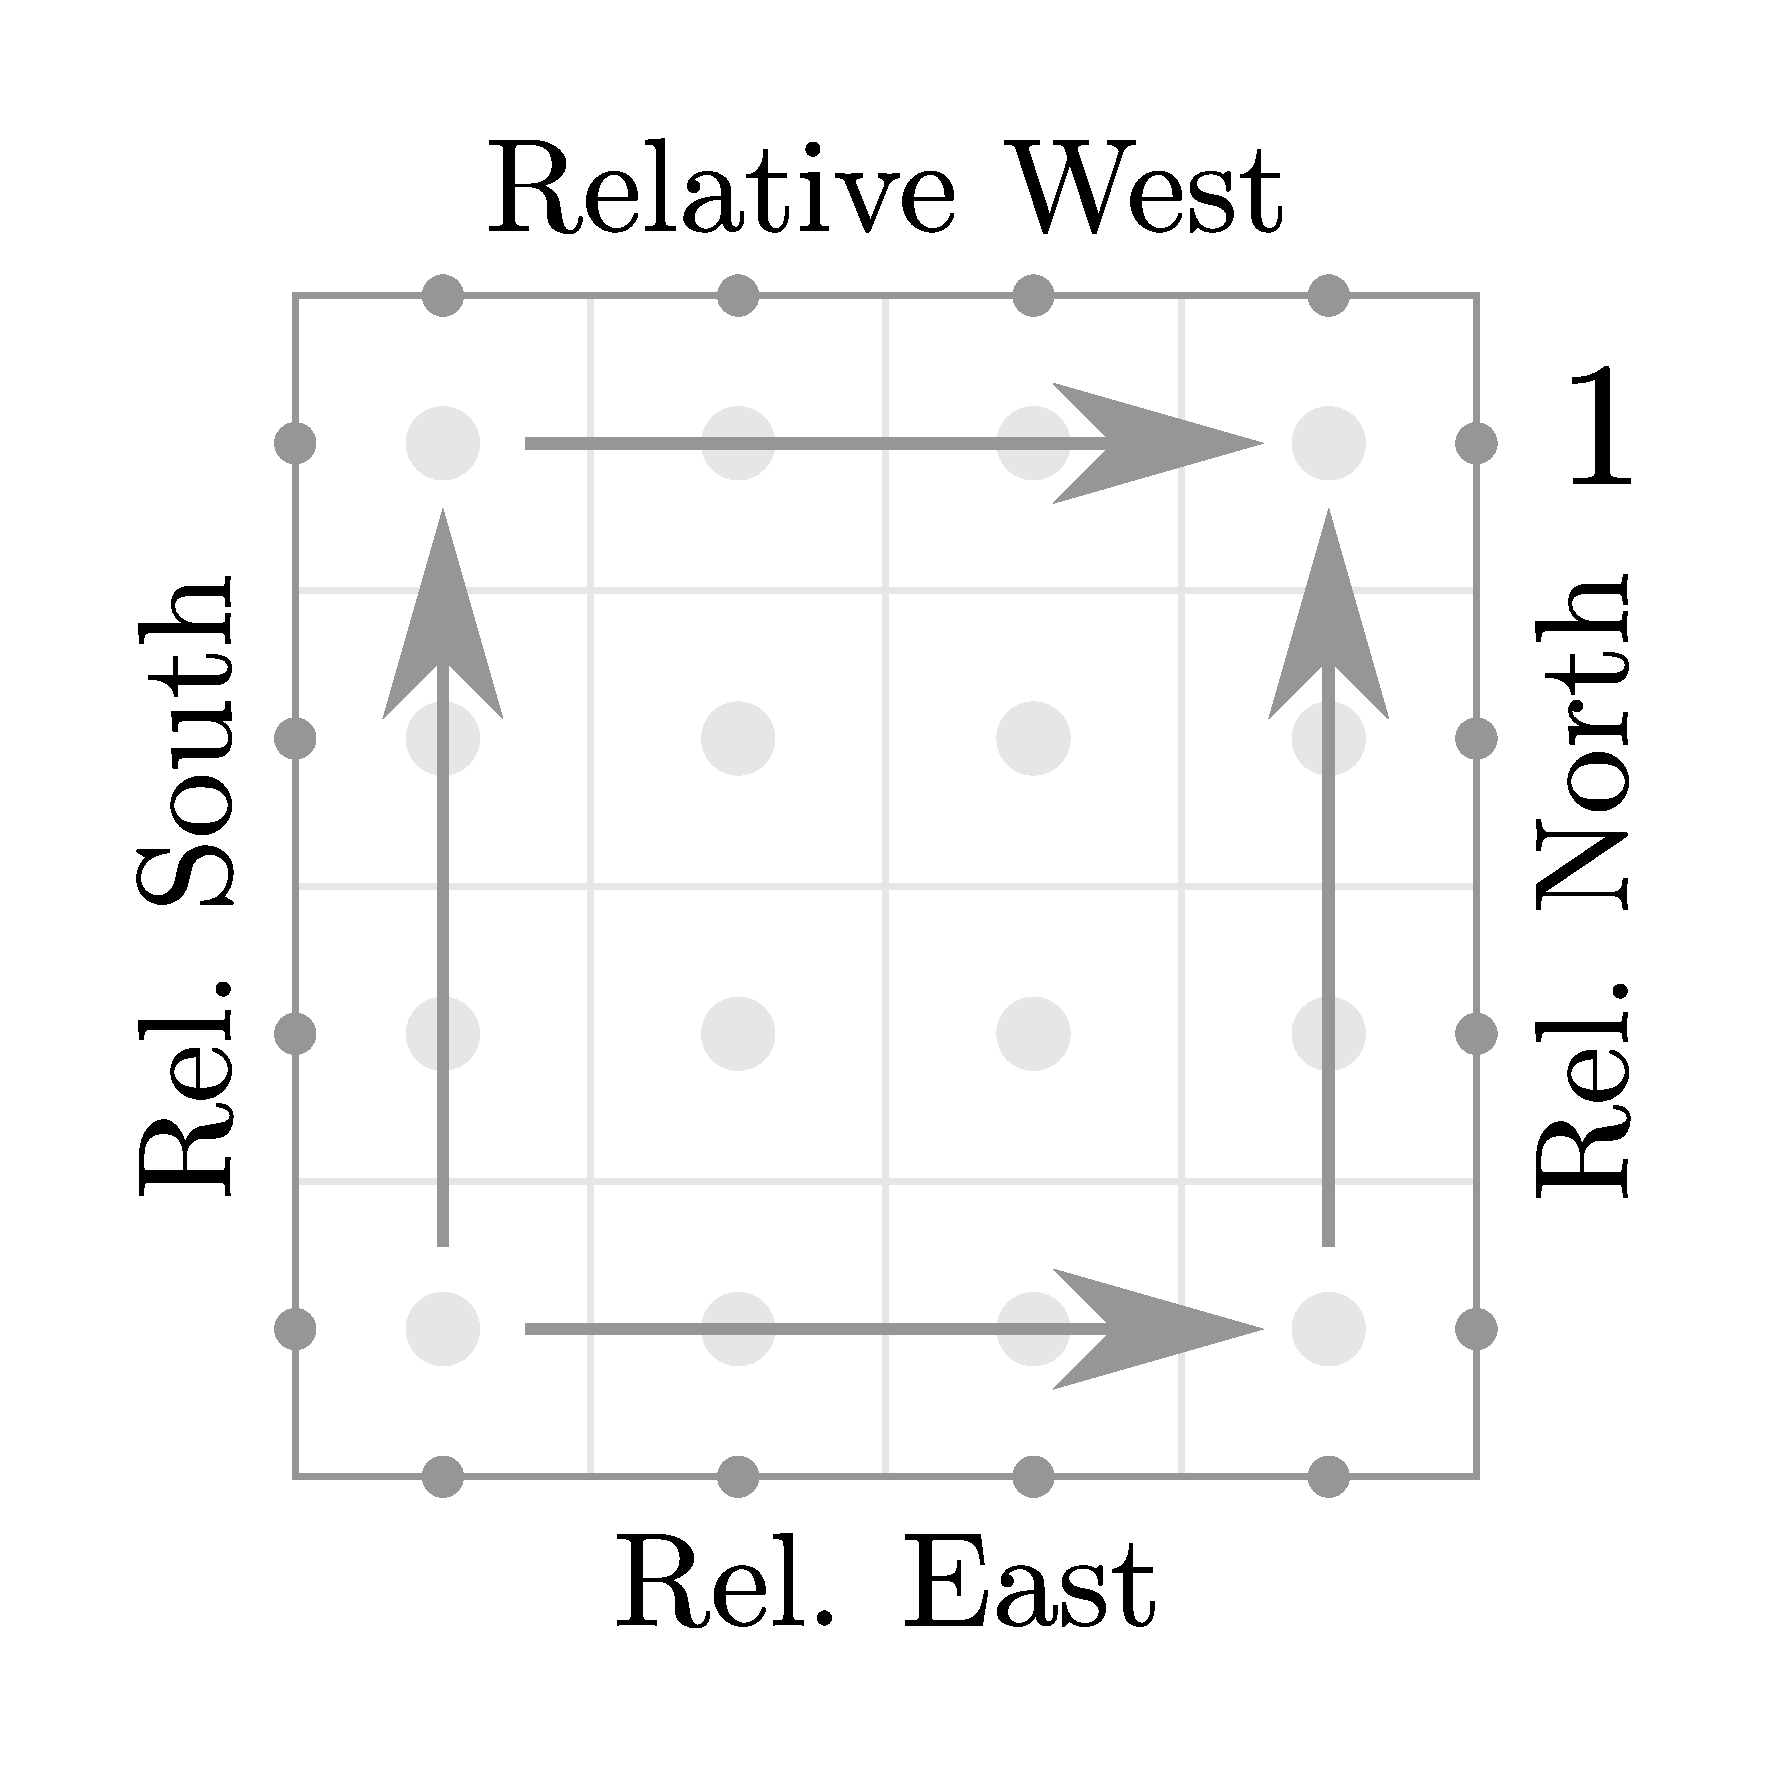
\includegraphics[width=\textwidth]{images/east1.pdf}
        \caption{East}
    \end{subfigure}
    \begin{subfigure}[b]{0.30\textwidth}
        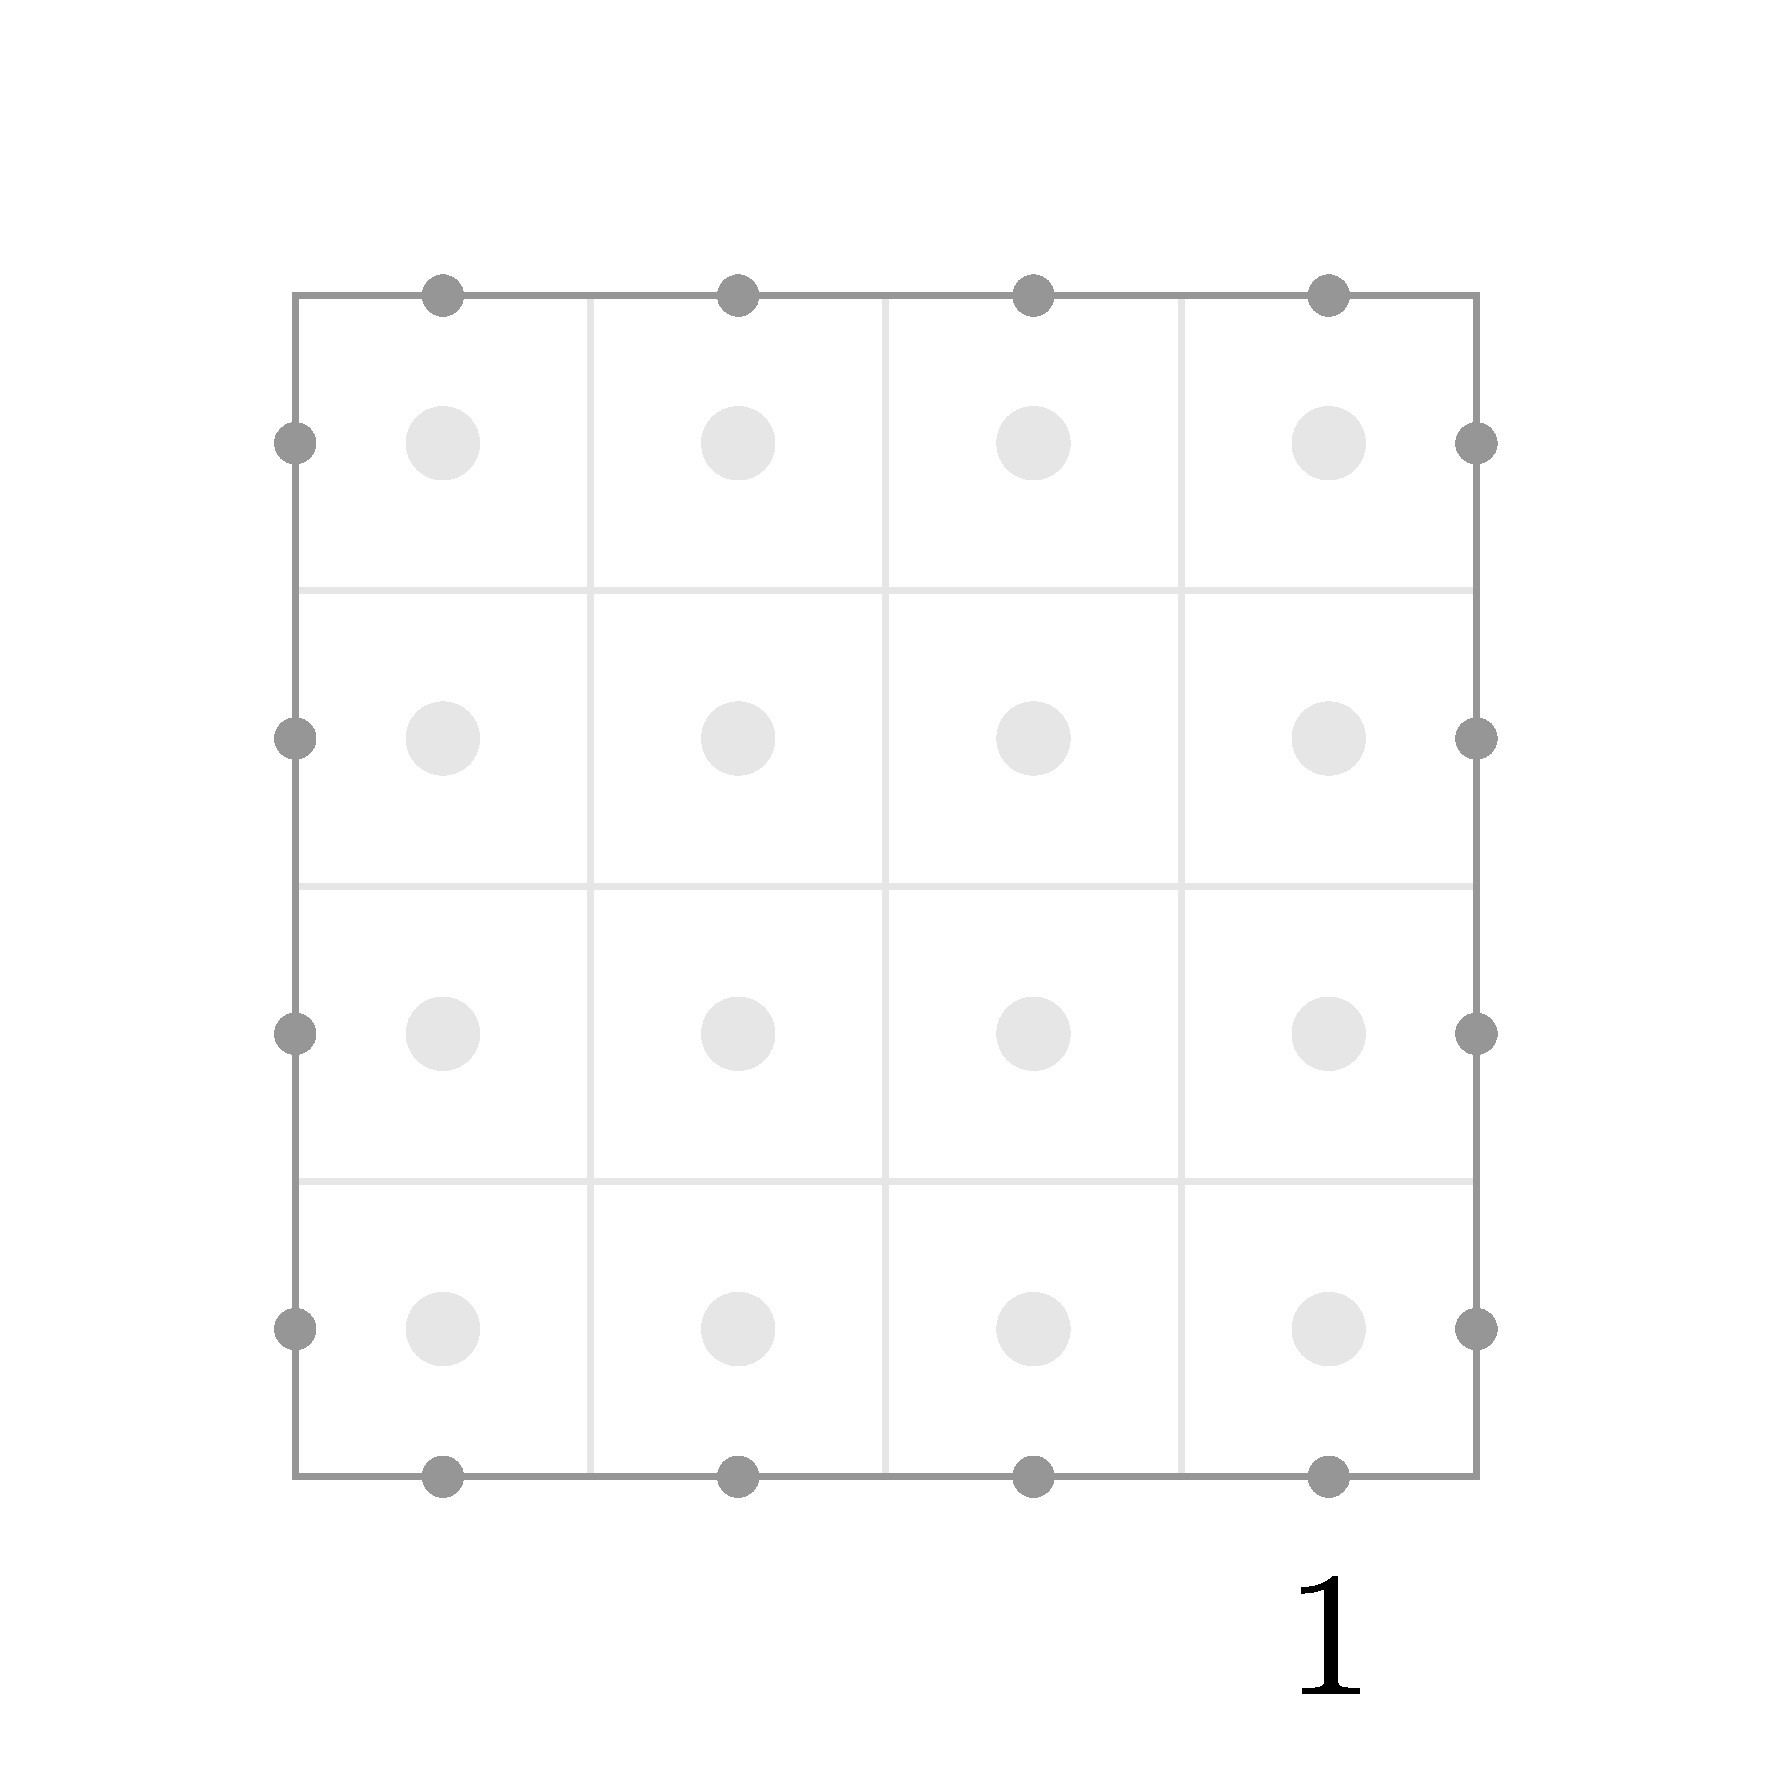
\includegraphics[width=\textwidth]{images/south1.pdf}
        \caption{South}
    \end{subfigure}
    \begin{subfigure}[b]{0.30\textwidth}
        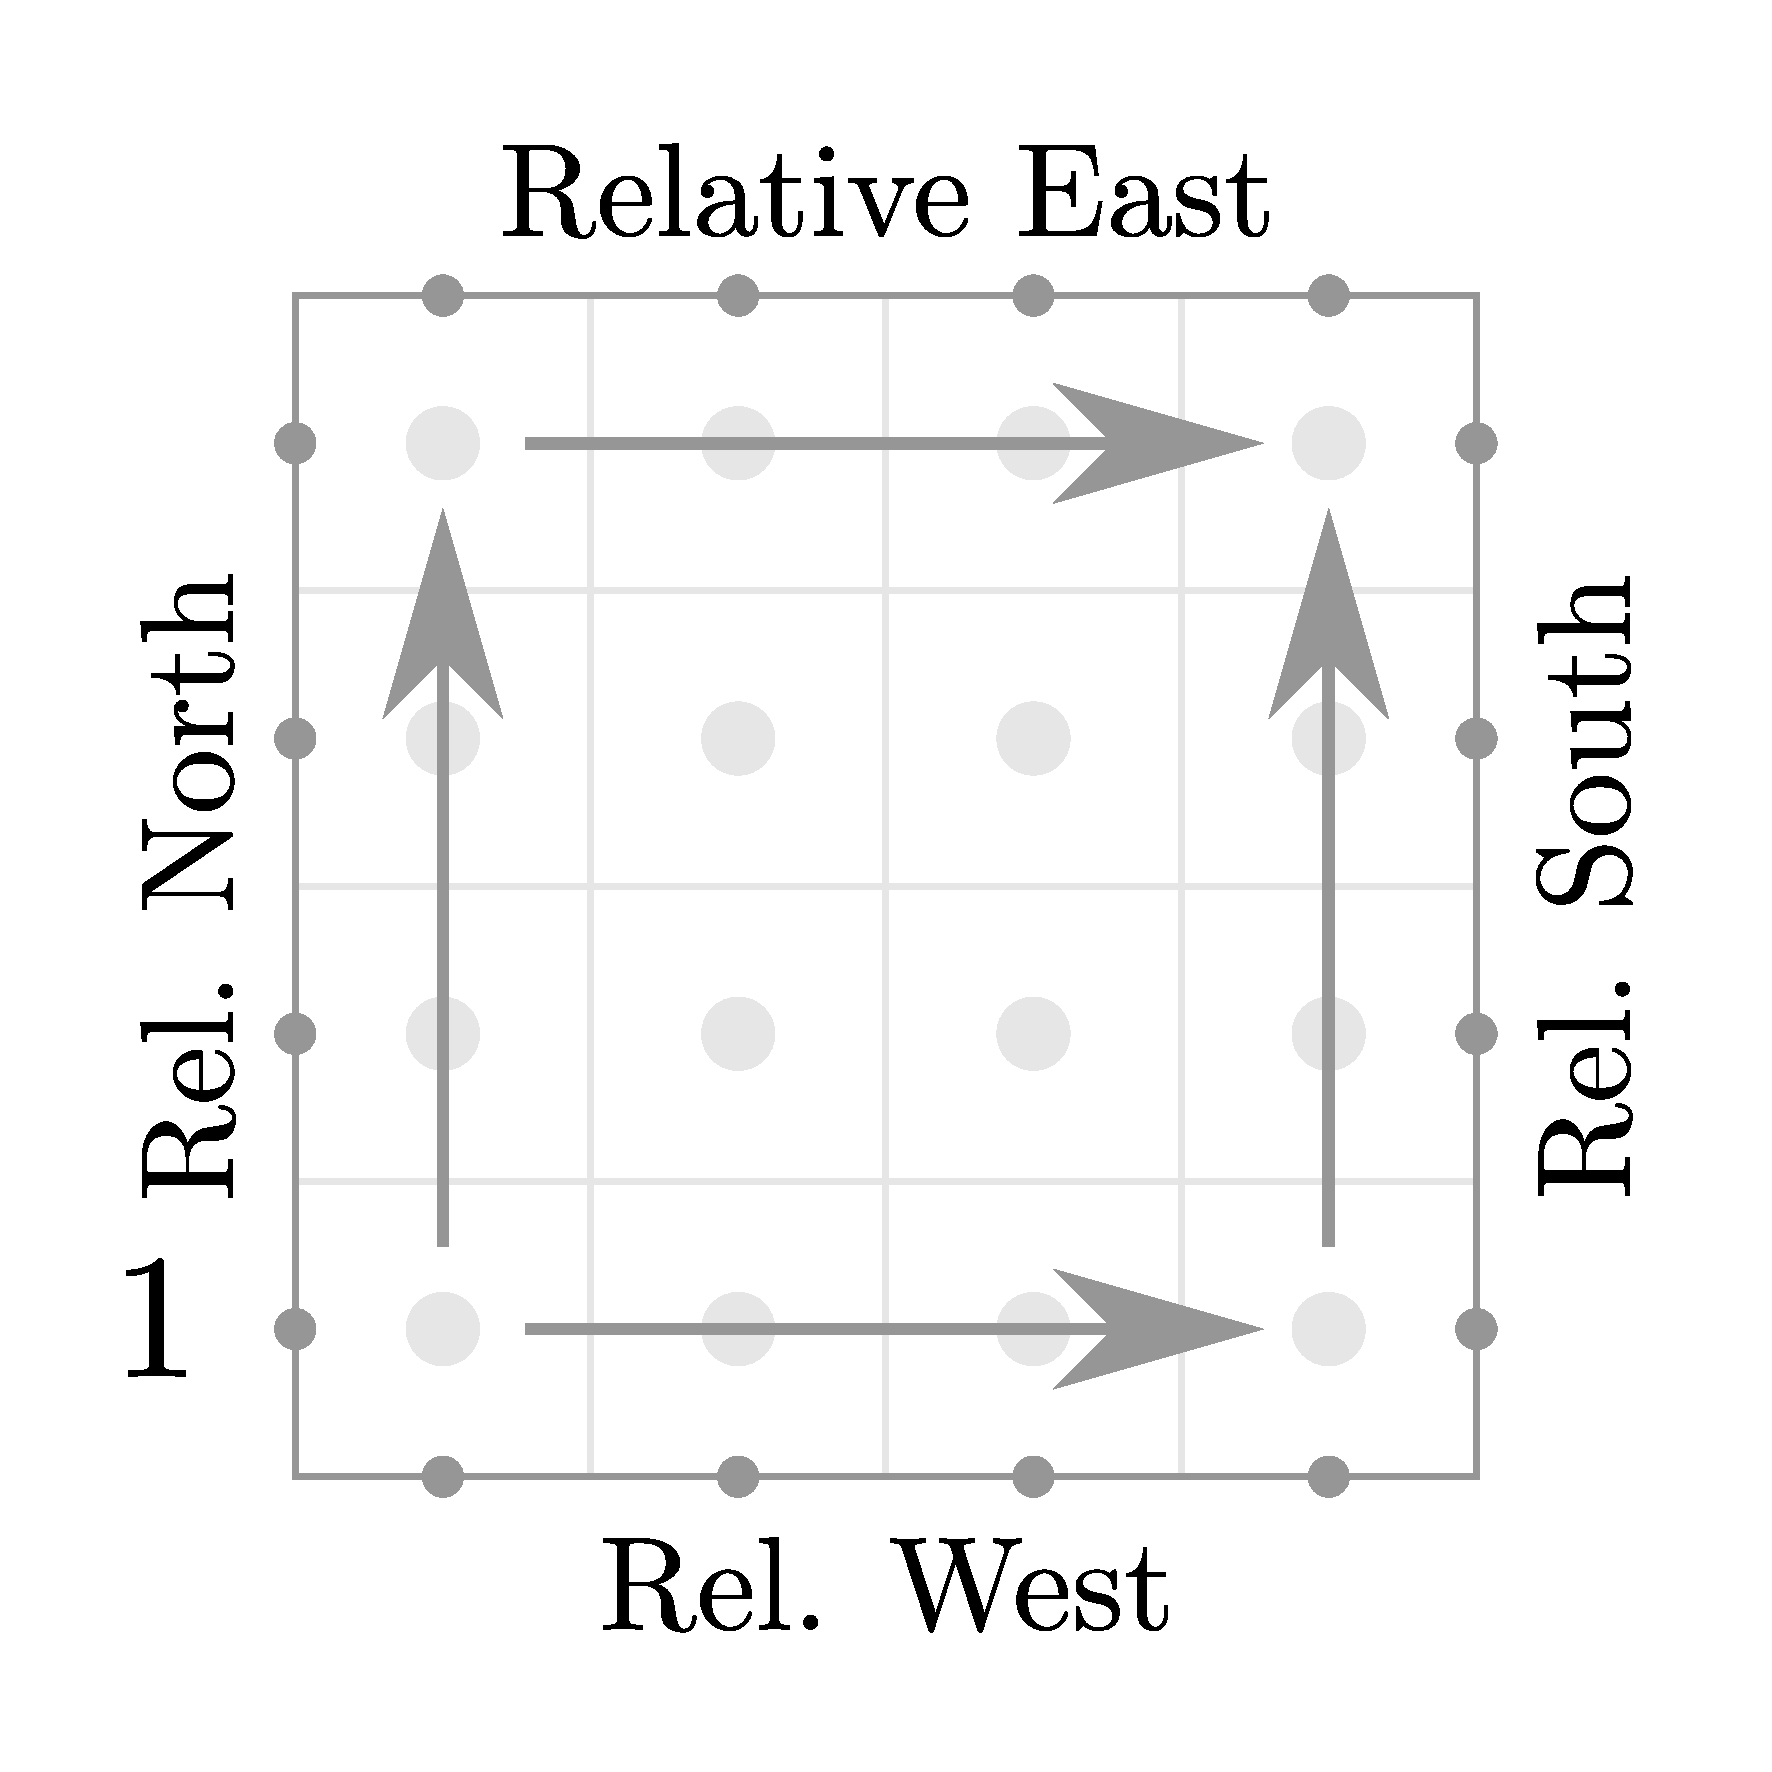
\includegraphics[width=\textwidth]{images/west1.pdf}
        \caption{West}
    \end{subfigure}

    \caption{Rotation}
    \label{rotation}
\end{figure}

We can get the coefficients for the blocks in the Schur complement matrix by
setting each $\gamma$ value along one side of the domain to $1$, and then reuse these coefficients 
for the interfaces on the other sides.

Let the north side be our canonical side. If we set each $\gamma$ value along the north interface to
$1$, we can save the resulting coefficients into four blocks. This is done in algorithm
\ref{getblocks}. We can reuse these blocks for the other interfaces, but the order of the columns 
and the rows in each block may be incorrect.

First, let's consider the order of the columns.
In part (a) of figure \ref{rotation}, the
first $\gamma$ value on the north interface is set to $1$. If we rotate this domain clockwise by $90$
degrees, that is equivalent to setting the last $\gamma$ value on the east interface to $1$. This
means that the order of the columns of our canonical blocks will be in the wrong order if we want to
reuse those blocks for the east interface. This is also true for the south interface. A table for
whether or not to reverse the order of the columns of the canonical blocks is given in table \ref{revcol} 
\begin{table}[H]
    \centering
\begin{tabular}{ cccc }
                   North & East & South & West \\ \hline
     False & True & True & False \\
\end{tabular}
    \caption{Reversal of columns}
    \label{revcol}
\end{table}
Next, let's consider the order of the rows. If we compare part (a) to part (b) in figure
\ref{rotation}, we can see that the consecutive ordering of the interface values (the arrows in
the figures) are pointing the opposite direction. This means that when we get each column of
coefficients for the north canonical block, the order of the rows of coefficients will be wrong when
we use them in the other interfaces. A completely worked out logic table for whether or not we need
to reverse the order of columns in each of the canonical blocks is given in table \ref{revrow}.
\begin{table}[H]
    \centering
\begin{tabular}{ r | cccc }
                  & North & East  & South & West \\ \hline
    North Block   & False & True  & True & False \\
    East  Block   & False & False & True & True  \\
    South Block   & False & True  & True & False \\
    West  Block   & False & False & True & True  \\
\end{tabular}
    \caption{Reversal of rows}
    \label{revrow}
\end{table}

\begin{algorithm}
\caption{}
\label{getblocks}
\begin{algorithmic}[1]
    \Procedure{getBlocks}{n}
    \State $\Omega()$ \Comment{Create empty domain}
    \State $\Omega.rhs \gets 0$
    \State $\Omega.northBoundary \gets 0$
    \State $\Omega.eastBoundary \gets 0$
    \State $\Omega.southBoundary \gets 0$
    \State $\Omega.westBoundary \gets 0$
    \State $NorthBlock(n*n)$ \Comment{Allocate blocks of size n*n}
    \State $EastBlock(n*n)$
    \State $SouthBlock(n*n)$
    \State $WestBlock(n*n)$
    \For{$i \gets 1,n$}
         \State $\Omega.northBoundary(i) \gets 1$
         \State $\Omega.\Call{solve}{ }$
         \State $NorthBlock(:,i) \gets \Omega.northBoundary - \Call{North}{\Omega}$
         \State $EastBlock(:,i) \gets -\Call{East}{\Omega}$
         \State $SouthBlock(:,i) \gets -\Call{South}{\Omega}$
         \State $WestBlock(:,i) \gets -\Call{West}{\Omega}$
         \State $\Omega.northBoundary(i) \gets 0$
    \EndFor

    \State \Return $NorthBlock, EastBlock, SouthBlock, WestBlock$
    \EndProcedure
\end{algorithmic}
\end{algorithm}
\paragraph{Algorithm}
The algorithm for quick matrix formulation will have three steps:
\begin{enumerate}
    \item Enumerate a set of interface structs
    \item Get coefficients for cannonical blocks
    \item For each interface struct, insert the blocks for that interface into the matrix
\end{enumerate}
Algorithm \ref{ifaces} shows how to enumerate a set of inteface structs. Each struct has 
$side$, $northIndex$, $southIndex$, and $westIndex$ fields. The $side$ field is which side of the
domain the inteface is on, and each index is relative to that side (see figure \ref{rotation}).

\begin{algorithm}[H]
\caption{}
\begin{algorithmic}[1]
    \Procedure{EnumerateIfaceStructs}{Domains}
    \State $ifaces \gets \emptyset$ \Comment{Set of interfaces to be processed}
    \ForAll{$\Omega \in Domains$}
        \For{$side \in \{North,East,South,West\}$}
            \If{$\Omega.hasNeighbor(side)$}
                \State $iface()$ \Comment{New iface object}
                \State $iface.side \gets side$
                \State $iface.northIndex \gets \Omega.getIndex(side)$
                \State $iface.eastIndex \gets \Omega.getIndex(\Call{Rotate}{side,90})$
                \State $iface.southIndex \gets \Omega.getIndex(\Call{Rotate}{side,180})$
                \State $iface.westIndex \gets \Omega.getIndex(\Call{Rotate}{side,260})$
                \State $ifaces.insert(iface)$
            \EndIf
        \EndFor
    \EndFor
    \State \Return $ifaces$
    \EndProcedure
\end{algorithmic}
    \label{ifaces}
\end{algorithm}
\begin{algorithm}[H]
\caption{Matrix Formulation}
\begin{algorithmic}[1]
    \Procedure{FormMatrix}{Domains}
    \State $ifaces \gets \Call{EnumerateIfaceStructs}{Domains}$
    \State $NorthBlock, EastBlock, SouthBlock, WestBlock \gets \Call{getBlocks}{n}$
    \State $A()$ \Comment{Allocate Matrix}
    \ForAll{$iface \in ifaces$} \Comment{Insert Blocks into Matrix}
        \State
        \State $reverseColumns \gets \Call{RevColTable}{iface.side}$
        \State $reverseRows \gets \Call{RevRowTable}{iface.side,North}$
        \State $j \gets iface.northIndex$
        \State $A.insertBlock(NorthBlock,j,j,reverseColumns,reverseRows)$
        \State
        \If{$\Omega.eastIndex \not= null$}
            \State $reverseRows \gets \Call{RevRowTable}{iface.side,East}$
            \State $i \gets iface.eastIndex$
            \State $A.insertBlock(EastBlock,i,j,reverseColumns,reverseRows)$
        \EndIf
        \State
        \If{$\Omega.southIndex \not= null$}
            \State $reverseRows \gets \Call{RevRowTable}{iface.side,South}$
            \State $i \gets iface.southIndex$
            \State $A.insertBlock(SouthBlock,i,j,reverseColumns,reverseRows)$
        \EndIf
        \State
        \If{$\Omega.westIndex \not= null$}
            \State $reverseRows \gets \Call{RevRowTable}{iface.side,West}$
            \State $i \gets iface.westIndex$
            \State $A.insertBlock(WestBlock,i,j,reverseColumns,reverseRows)$
        \EndIf
        \State
    \EndFor
    \State \Return $A$
    \EndProcedure
\end{algorithmic}
\end{algorithm}

\section{Handling Refinement}
We want the flux going out of the coarse cell to match the fluxes going into 
the fine cells.

\begin{figure}[H]
    \centering
    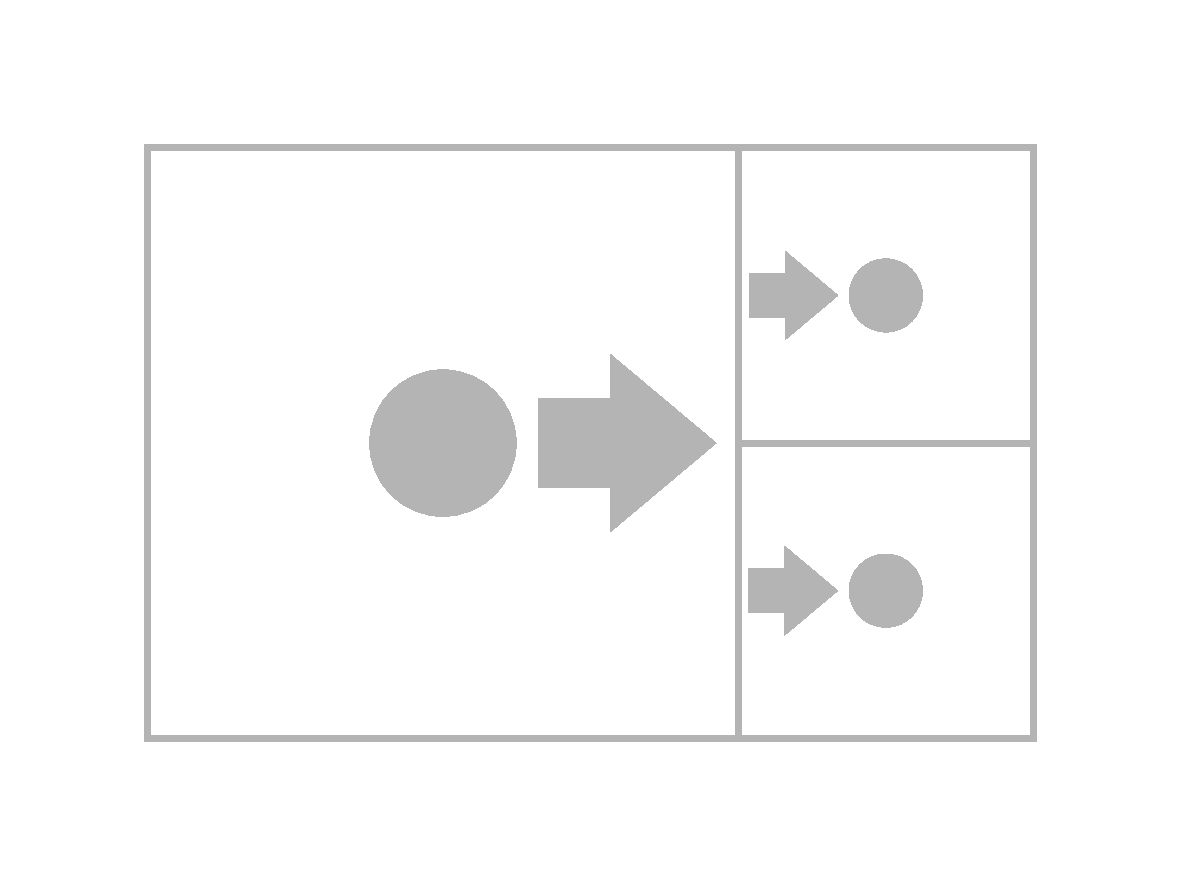
\includegraphics[width=4in]{images/amrflux.pdf}
    \caption{flux}
\end{figure}

We can represent this with the equation:

\begin{equation}
    \Phi_{c}=\Phi_{f_1}+\Phi_{f_2}
    \label{fluxconsv}
\end{equation}

\subsubsection*{Coming up with a stencil}
Lets say we want to find the ghost values for the coarse cell, the first fine cell, and the second
fine cell. Labeled $g_c$,$g_{f_1}$,and $g_{f_2}$, respectively.

\begin{figure}[H]
    \centering
    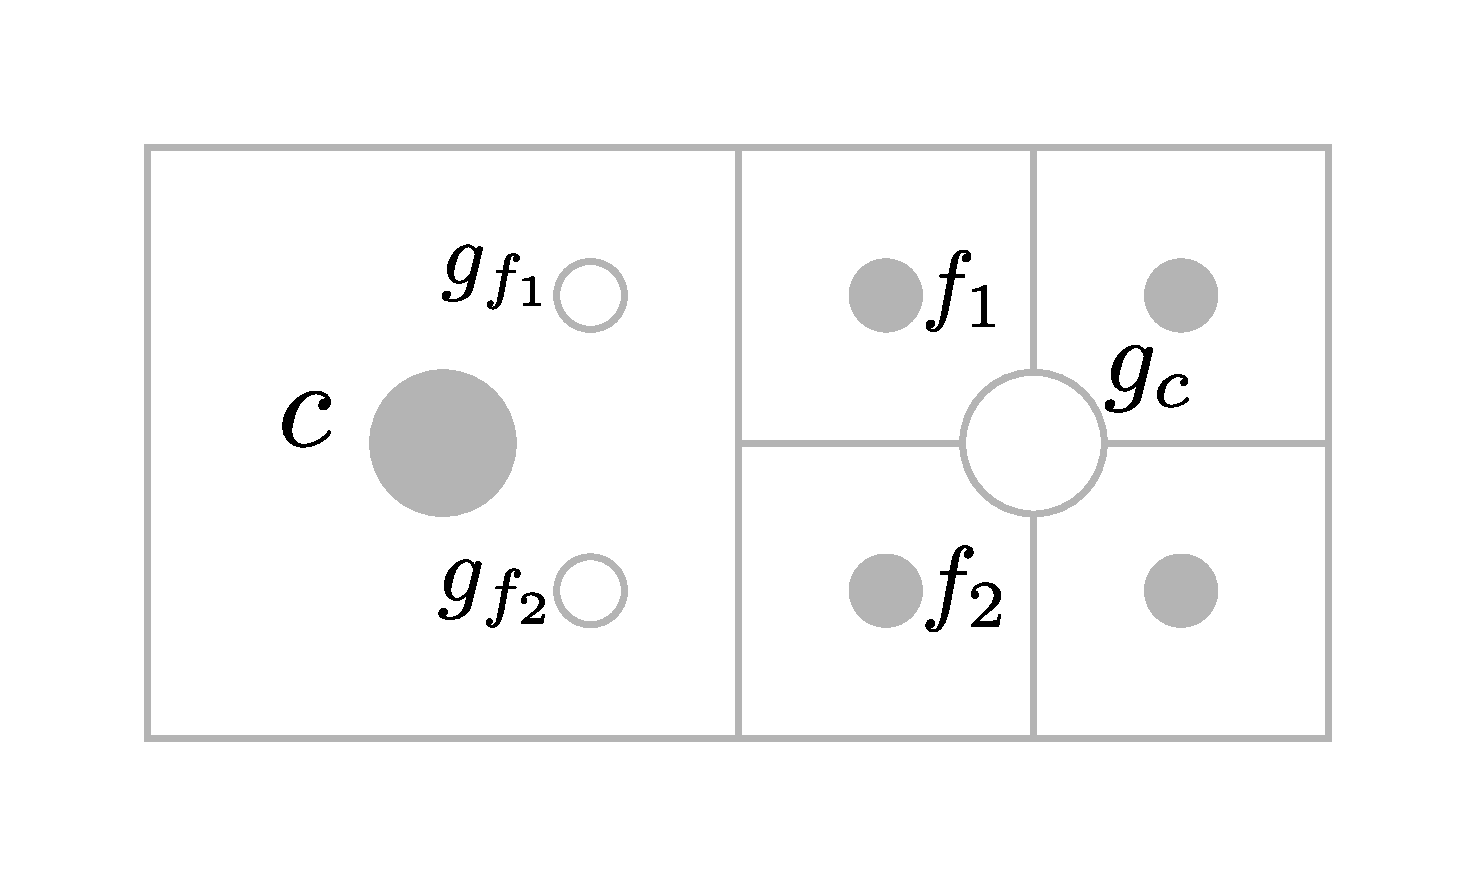
\includegraphics[width=4in]{images/ghost.pdf}
    \caption{ghost points}
\end{figure}

We can enforce flux conservation by interpolating to the fine ghost points, and then using equation
\ref{fluxconsv} to find the ghost point for the coarse cell.

The fluxes for each cell will be:
\begin{align}
    \Phi_c&=g_c-c\\
    \Phi_{f_1}&=f_1-g_{f_1}\\
    \Phi_{f_2}&=f_2-g_{f_2}
\end{align}

We can then solve for the value of $g_c$:

\begin{align}
    \Phi_{c}&=\Phi_{f_1}+\Phi_{f_2}\\
    g_c-c   &=f_1-g_{f_1}+f_2-g_{f_2}\\
    g_c     &=c+f_1-g_{f_1}+f_2-g_{f_2}
    \label{ghostconsv}
\end{align}

\subsubsection*{Bilinear interpolation}

Bilinear interpolation for the fine ghost points works, but error is not continuous.

TODO: Explain this and show an example

\subsubsection*{Quadratic interpolation}



\begin{figure}[H]
    \centering
    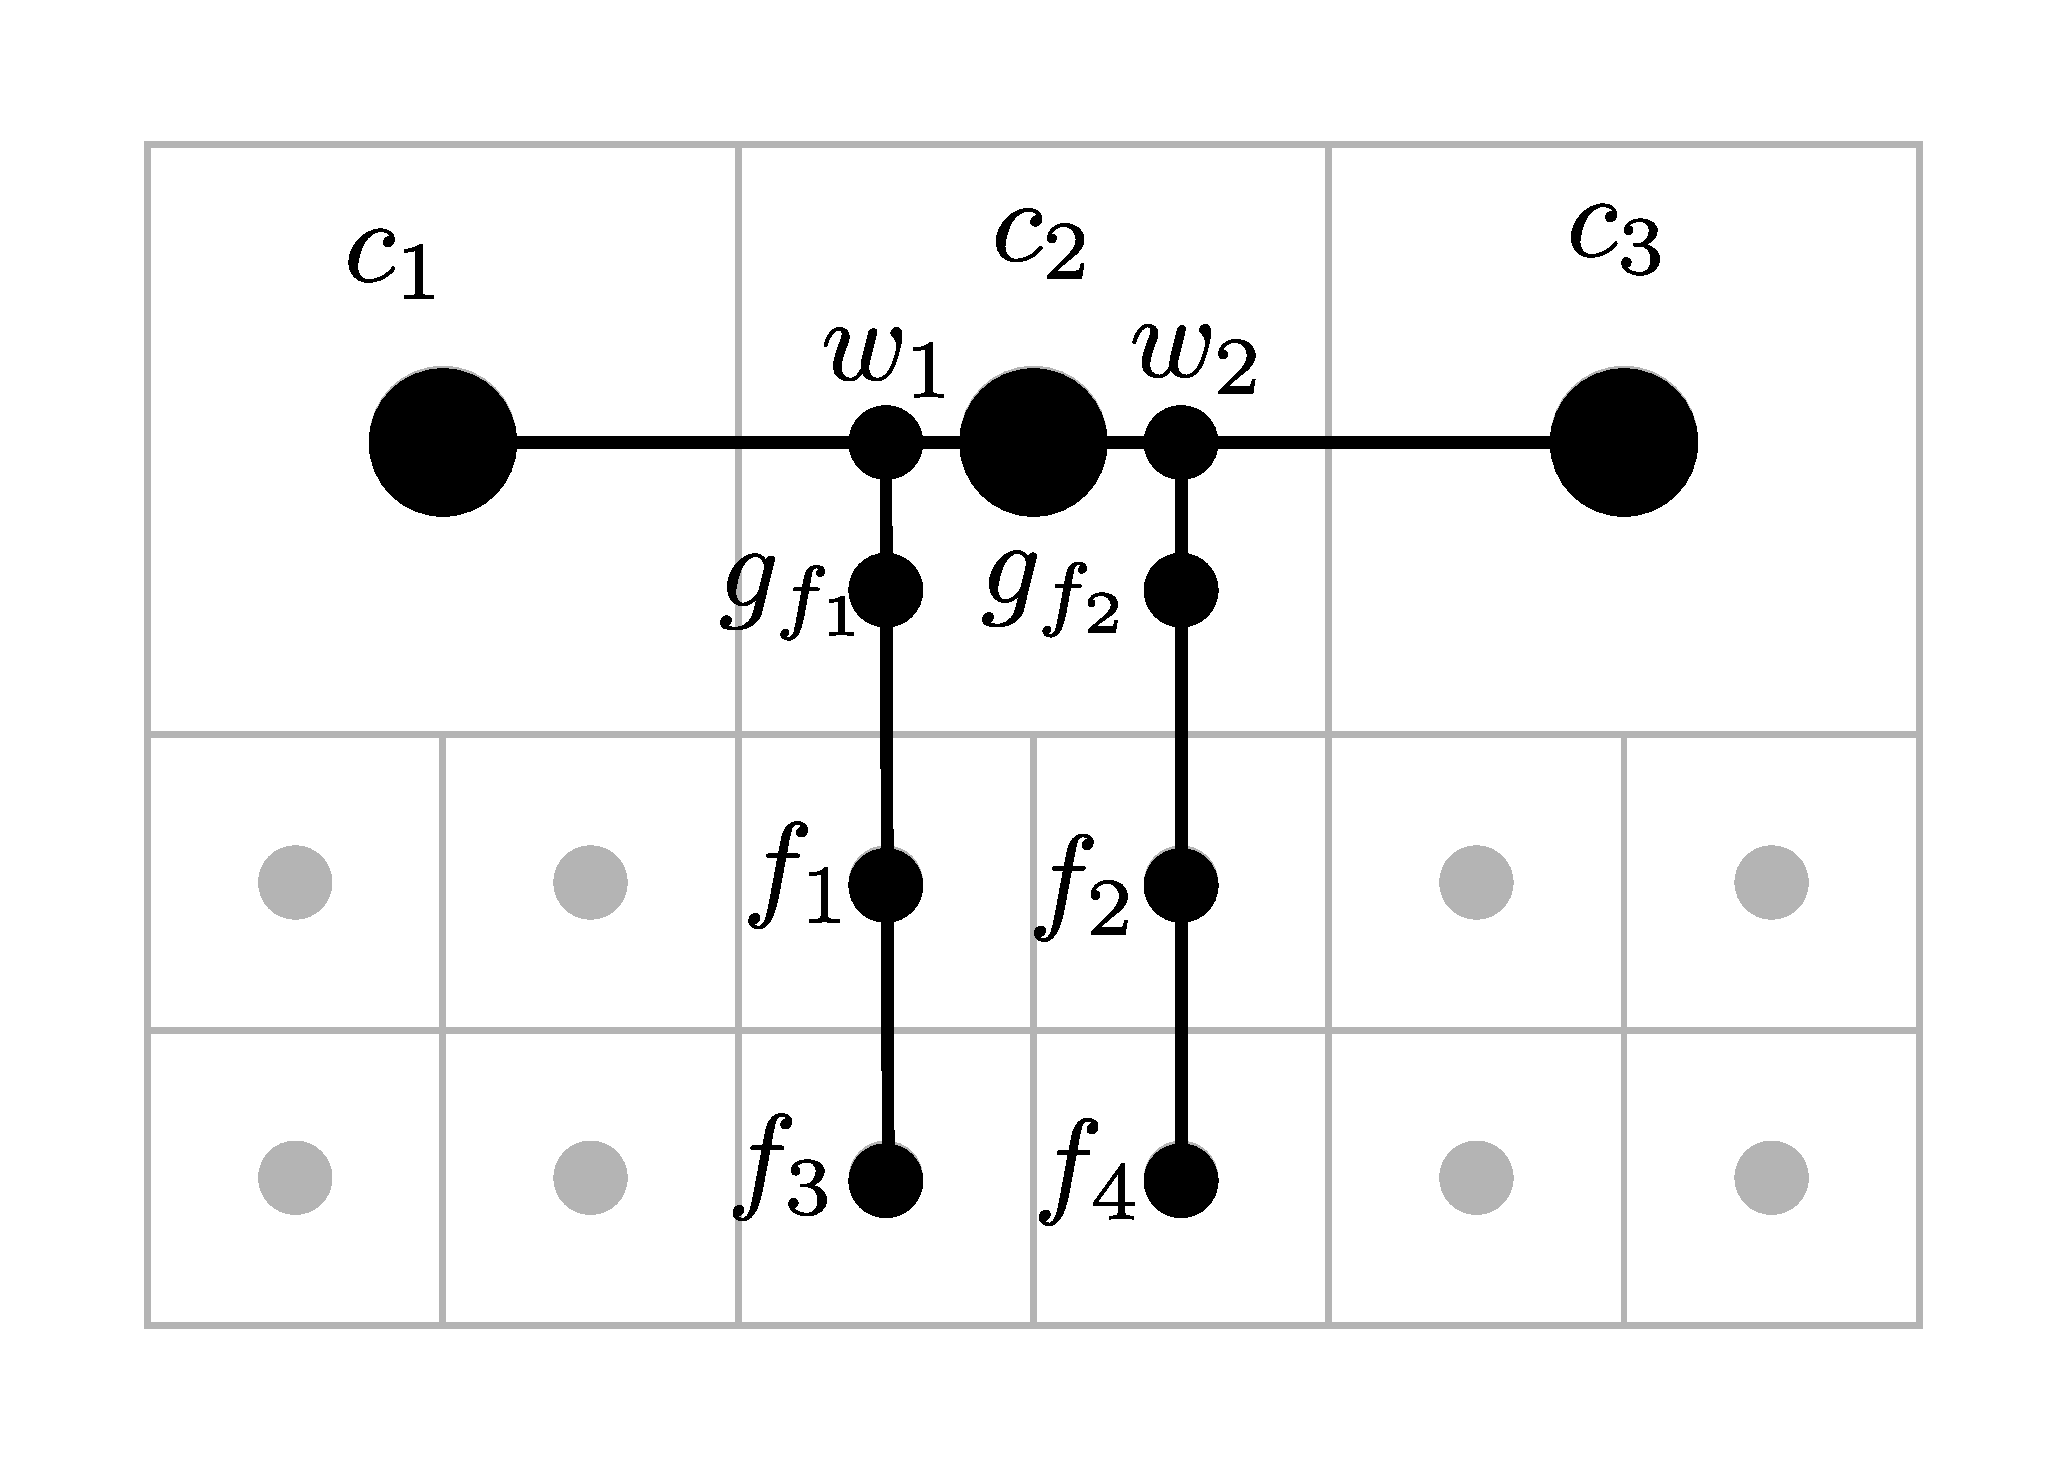
\includegraphics[width=5in]{images/quadstencil.pdf}
    \caption{flux}
\end{figure}

To find the value of $g_{f_1}$, we first use quadratic interpolation with the points 
$c_1$, $c_2$, and $c_3$ to interpolate to $w_1$:
\begin{equation*}
    w_1=\frac{5}{32}c_1+\frac{15}{16}c_2-\frac{3}{32}c_3
\end{equation*}
We then use quadratic interpolation with the points 
$w_1$, $f_1$, and $f_3$ to interpolate to $g_{f_1}$:
\begin{equation*}
    g_{f_1}=\frac{8}{15}w_1+\frac{2}{3}f_1-\frac{1}{5}f_3
\end{equation*}
Plug in the value for $w_2$, and we get the final equation for $g_{f_1}$:
\begin{equation*}
    g_{f_1}=\frac{1}{12}c_1+\frac{1}{2}c_2-\frac{1}{20}c_3 +\frac{2}{3}f_1-\frac{1}{5}f_3
\end{equation*}
The equation for $g_{f_2}$ is similar:
\begin{equation*}
    g_{f_2}=-\frac{1}{20}c_1+\frac{1}{2}c_2+\frac{1}{12}c_3 +\frac{2}{3}f_2-\frac{1}{5}f_4
\end{equation*}
Now that we have $g_{f_1}$ and $g_{f_2}$, we can use Eq. \ref{ghostconsv} to get the value of
the ghost point for the coarse cell, $g_{c_2}$:
\begin{align*}
    g_{c_2}&=c_2+f_1-g_{f_1}+f_2-g_{f_2}\\
    g_{c_2}&=c_2+f_1-\left(\frac{1}{12}c_1+\frac{1}{2}c_2-\frac{1}{20}c_3 +\frac{2}{3}f_1-
    \frac{1}{5}f_3\right)+f_2-\left(-\frac{1}{20}c_1+\frac{1}{2}c_2+\frac{1}{12}c_3
    +\frac{2}{3}f_2-\frac{1}{5}f_4\right)\\
    g_{c_2}&=-\frac{1}{30}c_1-\frac{1}{30}c_3+\frac{1}{3}f_1+\frac{1}{3}f_2+\frac{1}{5}f_3+
    \frac{1}{5}f_4
\end{align*}
\end{document}
